%%% template.tex
%%%
%%% This LaTeX source document can be used as the basis for your technical
%%% paper or abstract. Regardless of the length of your document, the commands
%%% are all the same.
%%% 
%%% The "\documentclass" command is the first command in your file. If you want to 
%%% prepare a version of your article with line numbers - a "review" version - 
%%% include the "review" parameter:
%%%    \documentclass[review]{acmsiggraph}
%%%

\documentclass[review]{acmsiggraph}

\usepackage{amsfonts}
\usepackage{amsmath}
%\usepackage{algorithm}
\usepackage[noend]{algpseudocode}
\usepackage[linesnumbered,ruled]{algorithm2e}
\usepackage{chngpage}
\usepackage{tabularx}
\usepackage{multirow}

\usepackage{graphicx}
\usepackage{caption}
\usepackage{subcaption}


%%% Title of your article or abstract.

\title{Rig Space Retargeting}

\author{Jaewon Song, Roger Blanco i Ribera, Kyungmin Cho, Byungkuk Choi, J.P.Lewis, Mi You, Junyong Noh}
\pdfauthor{Jaewon Song}

%%% Used by the ``review'' variation; the online ID will be printed on 
%%% every page of the content.

\TOGonlineid{0264}

% User-generated keywords.

\keywords{Character animation, Rig, Motion capture, Spacetime Optimization}

% With the "\setcopyright" command the appropriate rights management text will be added
% to your document.

%\setcopyright{none}
%\setcopyright{acmcopyright}
%\setcopyright{acmlicensed}
\setcopyright{rightsretained}
%\setcopyright{usgov}
%\setcopyright{usgovmixed}
%\setcopyright{cagov}
%\setcopyright{cagovmixed}
%\setcopyright{rightsretained}

% The year of publication in the "\copyrightyear" command.

\copyrightyear{2016}

%%% Conference information, from the completed rights management form.
%%% The "\conferenceinfo" command has two parameters: 
%%%    - conference name
%%%    - conference date and location
%%% The "\isbn" field includes the year and month after the article ISBN.

\conferenceinfo{SIGGRAPH 2016 Posters}{July 24-28, 2016, Anaheim, CA} 
\isbn{978-1-4503-ABCD-E/16/07} 
\doi{http://doi.acm.org/10.1145/9999997.9999999}

\begin{document}


%%% This is the ``teaser'' command, which puts an figure, centered, below 
%%% the title and author information, and above the body of the content.

 \teaser{
   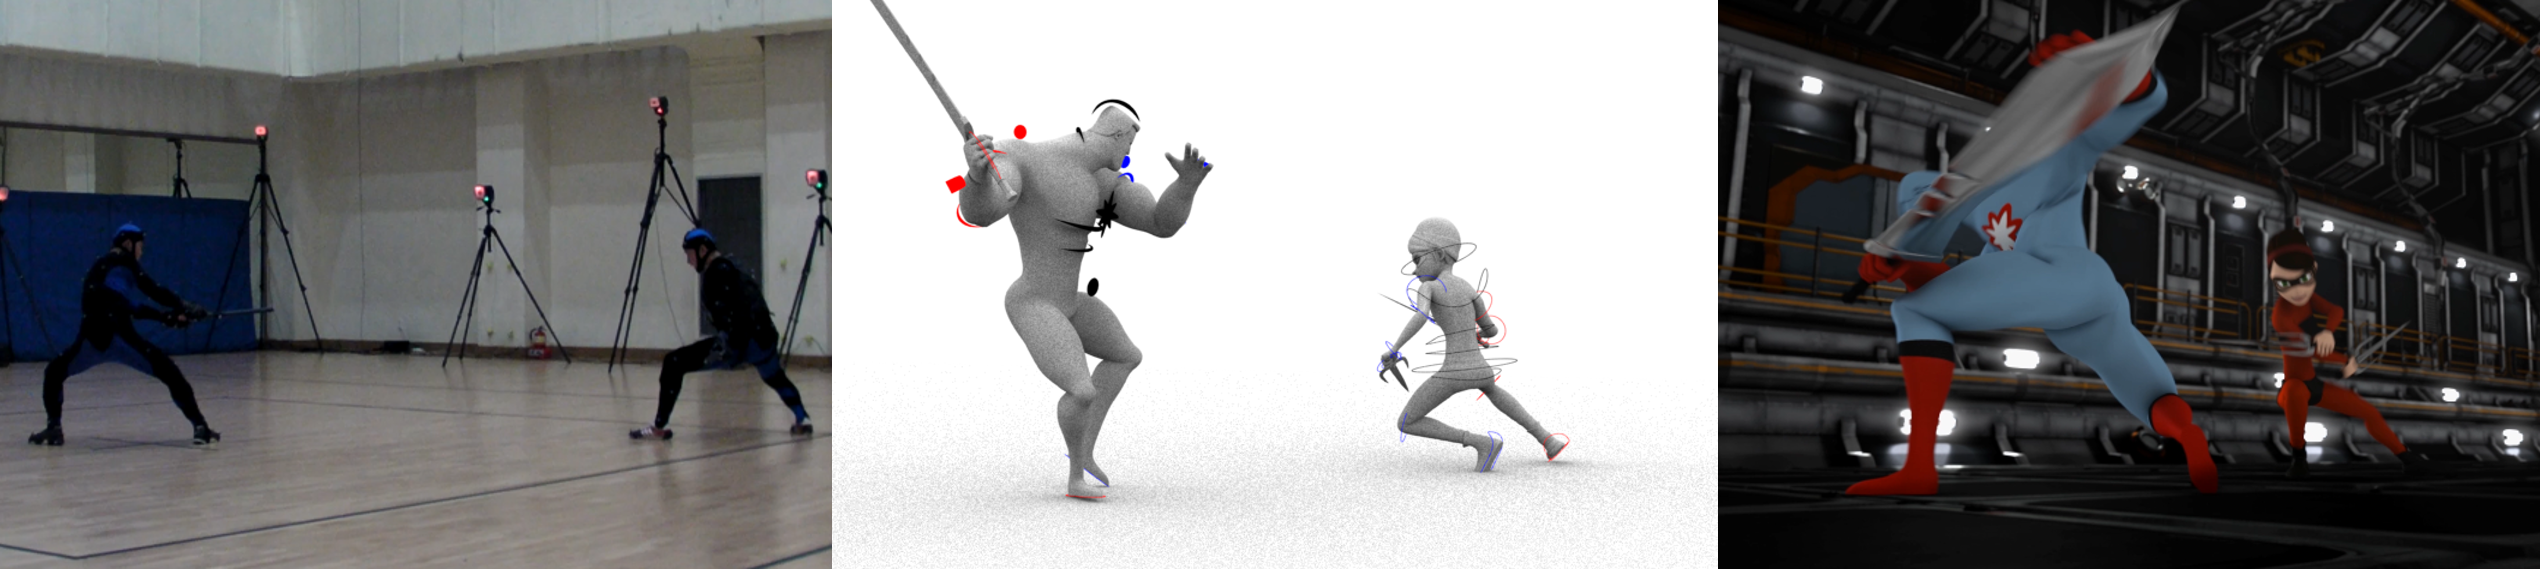
\includegraphics[height=1.5in]{images/teaser}
   \caption{Overall process of our rig space retargeting is applied for the production pipeline. (left) Motion capture (middle) Rig space mapping result with our method (right) Final animation by artist}
 }

\maketitle
\def \SE {$SE(3)\times \ldots \times SE(3)$}
\def \se {$\mathfrak{se}(3)\times \ldots \times \mathfrak{se}(3)$}

\begin{abstract}

We propose a novel inverse motion mapping method for the parameters in \textit{rig space} - the space continuously spanned by the control parameters commonly employed for the setup of a character. 
Since the rig space is the user interface designed to help an artist interact with a character in various ways for the creation of animation, it is difficult to provide a general solution for the inverse rig mapping that can work for arbitrary rigs.
Our inverse motion mapping method maps the existing motion data into the rig space parameters based on spacetime optimization. The technique does not require any user provided priors such as manual identification of correspondences or example motions created by an artist.
We first perform analysis of the rig of a character and generate a correlation map between the rig space and the skeleton space. Based on the correlation map, we divide the full body rig into a set of mutually independent groups of the body parts to change the full body optimization problem into a set of sub-body optimization problems. This allows fast convergence of the computation. 
We also propose a novel representation for rigid skeletal motion, which is defined as a curve on the \SE{} Lie group in order to achieve accurate measurement of the distance during the optimization process. Due to the difficulty involved in the parameter optimization on a curved manifold of Lie group, we perform the optimization after the linearization of the manifold into the Lie algebra \se{} which is the vector space of Lie group. Additionally, the artist can assign constraints during the optimization to specify the working style and to handle commonly occurring motion mapping artifacts such as self-penetration. The results show that our motion mapping can be applied robustly to various rig types and therefore increase the productivity in the professional production pipeline.

\end{abstract}


%
% The code below should be generated by the tool at
% http://dl.acm.org/ccs.cfm
% Please copy and paste the code instead of the example below. 
%
%\begin{CCSXML}
%<ccs2012>
%<concept>
%<concept_id>10010147.10010371.10010382</concept_id>
%<concept_desc>Computing methodologies~Image manipulation</concept_desc>
%<concept_significance>500</concept_significance>
%</concept>
%<concept>
%<concept_id>10010147.10010371.10010382.10010236</concept_id>
%<concept_desc>Computing methodologies~Computational photography</concept_desc>
%<concept_significance>300</concept_significance>
%</concept>
%</ccs2012>
%\end{CCSXML}
%
%\ccsdesc[500]{Computing methodologies~Image manipulation}
%\ccsdesc[300]{Computing methodologies~Computational photography}

\begin{CCSXML}
<ccs2012>
<concept>
<concept_id>10010147.10010371.10010352</concept_id>
<concept_desc>Computing methodologies~Animation</concept_desc>
<concept_significance>500</concept_significance>
</concept>
<concept>
<concept_id>10010147.10010371.10010352.10010238</concept_id>
<concept_desc>Computing methodologies~Motion capture</concept_desc>
<concept_significance>300</concept_significance>
</concept>
<concept>
<concept_id>10010147.10010371.10010352.10010380</concept_id>
<concept_desc>Computing methodologies~Motion processing</concept_desc>
<concept_significance>100</concept_significance>
</concept>
</ccs2012>
\end{CCSXML}

\ccsdesc[500]{Computing methodologies~Animation}
\ccsdesc[300]{Computing methodologies~Motion capture}
\ccsdesc[100]{Computing methodologies~Motion processing}
%
% End generated code
%

% The next three commands are required, and insert the user-generated keywords, 
% The CCS concepts list, and the rights management text.
% Please make sure there is a blank line between each of these three commands.

\keywordlist

\conceptlist

\printcopyright

\section{Introduction}

Artists often utilize real motion reference in the process of creating an animation to understand the key to successfully deliver certain actions and poses by working through the gathered examples. 
Even for highly exaggerated stylistic motion, the essential body mechanics transpire through the animation. 
This touch of reality, learned from the study of real life movements is essential to animate a believable movement. 
As the word implies, however, a reference is simply a starting point. 
The poses and timing information obtained from the reference will require most of the times the introduction of significant alterations in order to increase the appeal of the animation or fix the parts that did not translate well into the animation. 
Nonetheless, the little touch of reality insufflated into the animation through the reference strengthens the animation and reinforces its believability. 
Therefore, it would only seem natural to use motion data directly as a starting point of the animation process.

Despite these benefits, it is often considered difficult to apply motion data in keyframe animation pipeline because common methods of manipulating motion data are different from the process of production. 
Common methods typically edit the joint directly or rely on advanced motion editing techniques such as motion warping\cite{witkin1995motion} or motion stylization\cite{hsu2005style}. 
However, these methods are difficult to apply to animation pipeline because artists are trained to create character motion by character rig.
Rig, a control structure that allows to produce the motion of a 3D character, plays a key role in the animation production pipeline. 
A well-designed rig understands how an artist interacts with a character, provides an easy and efficient solution to produce complex motion,  and increases the productivity in animation generation\cite{mclaughlin2011character,orvalho2012facial}. 
Therefore, it would be an attractive idea to manipulate motion data with an artist-friendly rig. 
In this paper, we propose a novel mapping method from motion data to a general character rig. 
Our method can be seamlessly applied to the current animation production pipeline, and improve the efficiency in creating animation contents by directly mapping the existing motion data into parameters of character rig.

\begin{figure}[ht]
  \centering
  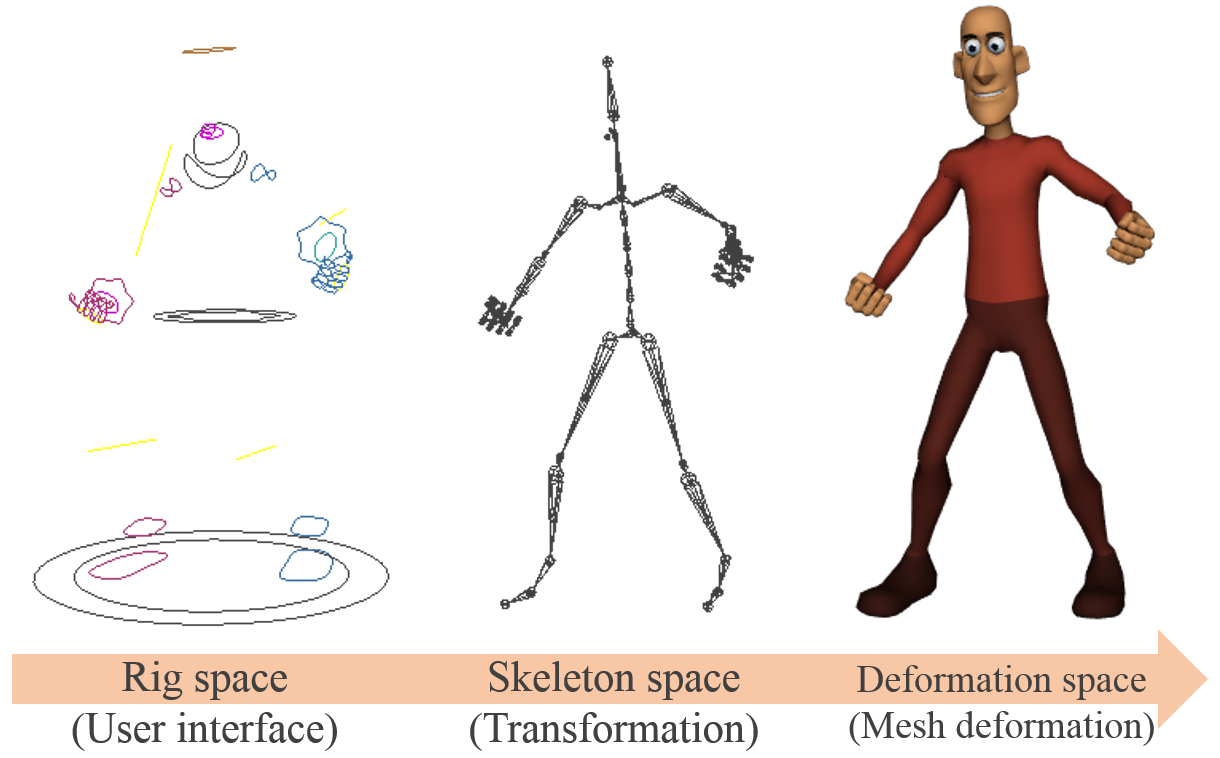
\includegraphics[width=1.0\linewidth]{images/rigLayer}
  \caption{Three layers of a character rig. The user interface layer controls the transformation layer, and the transformation layer in turn controls the skin deformer layer.}
  \label{fig:rigLayer}
\end{figure}

A character rig is composed of three layers\cite{orvalho2012facial} as shown in Figure \ref{fig:rigLayer}. 
The rig space, which is the user interface layer provides the artist with an interface that can control the skeleton space. 
In the skeleton space, the pose of a character is determined through the rigid body transformations applied to the hierarchical skeleton. 
Finally, the deformation layer deforms the character body by considering the correlation between the skeleton and the mesh vertices. Because our motion mapping occurs between the skeleton space and the rig space, we will not focus on the deformation layer in this study.

Artists are familiar with the rig space parameters and manipulate them skillfully for creation or editing of animation. 
However, this also means that the determination of the rig space depends on various factors such as the work preference of a specific artist, a desired rigging style, and the structure of a given character. Therefore, it is difficult to generally describe how the pose of a character can be represented in some optimal way, leading to multiple solutions for a single pose. 
Although such flexibility can help artists select preferred rig parameters depending on the task, it can cause ambiguity in the mapping process. 

Due to the aforementioned difficulties, professional artists often rely on manual identification of correlated operations between the skeleton space and the rig space in order to map motion data into the rig space parameters\cite{palamar2013mastering,DigitalTutor2013}. 
However, this approach suffers from a couple of drawbacks. 
First, as the mapping is performed on the positions and the orientations of the rig controllers, it is not clear how to handle user defined rig parameters that are often responsible for the generation of complex motions. 
Second, the manual process has to be repeated for a new character rig, making the process not well-scalable for a large scale production. 
Recently, Holden et al.\shortcite{holden2015learning} proposed an inverse rig mapping method based on a regression model, which incorporates example keyframe motion data prepared by an artist. 
Although this method works well with proper examples, it is often laborious to generate perfect example animations per each rig type.
%and the result of the inverse mapping can be biased toward the provided example data.

We propose an optimization-based inverse motion mapping method that does not rely on any manual specification of correspondences or prior data. 
Our inverse mapping problem finds the optimal rig parameters that minimize the distance between the pose generated by the rig parameters and the pose of the input motion. 
We first perform the rig analysis process that automatically groups the skeleton and the rig parameters, where each group has mutually independent rig operations with each other. 
Based on these groups, we divide the problem into a set of sub-problems and efficiently perform the optimization.

We also propose a novel skeletal representation on the $SE(3)$ Lie group manifold to measure the distance accurately between the poses during the optimization process. 
Mathematically, rigid body rotations or translations are members of the special Euclidean group $SE(3)$\cite{murray1994mathematical}, and therefore, the skeletal pose with multiple rigid body segments can be expressed as a point on the Lie group \SE. 
Geometrically, the Lie group \SE{} is a curved manifold, and therefore, the measure of the distance between two poses corresponds to the geodesic distance of the two points on the manifold. 
To overcome the difficulty of directly minimizing the geodesic distance, we linearize the Lie group \SE{} motion into the vector space which is the Lie algebra \se{}. We then perform our optimization as a linear programming.

During the optimization stage, we solve the ambiguity arising in the mapping process by regularizing the rig parameters. 
An artist who utilizes the rig would choose the most efficient rig parameters for a given animation task, based on his/her experiences and skills. 
This implies that the optimality of the rigging depends on the working style of the individual animator. 
However, a rigger who creates the rig would prefer a solution that results in minimum differences of sparse rig parameters. 
We opt to perform the regularization of the rig parameters to obtain sparse solutions. 
In addition, we allow the artist to additionally specify constraints on the rig parameters, to make the parameters converge toward the direction that complies with the artist's intention. 
This can solve errors frequently occurring in the motion mapping process such as self-penetration. 
We demonstrate the efficiency and usability of our method by performing the mapping onto various rigs and also show how seamlessly our approach can be applied to the production pipeline.




%\subsection{prev}
%Rig, which is defined as a control method to produce the motion of  a 3D character[V.Orvalho,2010], plays a key role in the animation production pipeline. Well designed rig understands how an artist interacts with a character, provides an easy and efficient solution to produce complex motion and thus, improve the productivity in animation generation\cite{mclaughlin2011character}.
%
%In this paper, we propose a novel inverse mapping method from motion data to general character rig.
%Our method can be seamlessly applied to current animation production pipeline, and improve the efficiency (in motion generation and editing) by directly mapping the existing motion data into parameters of character rig.
%Due to the effectiveness, the idea of using rig with motion data got attention in real production too.
%
%Character rig has 3 levels of data flow structure as shown in Figure \ref{fig:rigLayer}\cite{orvalho2012facial}. The top level called user interface layer provides an animator the interface which can control the transform layer. The transform layer decides the character pose through the rigid body transformation of hierarchical skeleton.
%Finally, the deformation layer shows character animation by deforming the character body considering the correlation between the skeleton and mesh vertices. 
%
%Here, we define the rig space as the user interface layer which is composed of various rig parameters that are controlled by the animator to produce character motion.
%The motion data is represented in skelton space, which is defined as skeleton parameters in transform layer. Since the inverse motion mapping problem is held in the skeleton space and the rig space, we are not going to handle the deformation layer directly.
%
%From the fact that the rig space parameters are directly used by artist(animator), it is important(valuable) and useful space for editing and modifying process in real animation production.
%
%However, the rig space is an abstract space. The direct interaction with an artist makes rig space dependent on character structure, work preference of animator, and rigging style of rigger, and thus, it is difficult to generally describe how rig space parameters decide the character pose.
%
%Due to the difficulties described above, a general approach of mapping motion data into rig space parameters is manually defining the correlation between the skeleton space and the rig space.[Maya][Animbinder][DigitalTutor]
%However, this requires a repetitive manual process on new rig, and only the simple mapping that uses the position and the orientation constraint is applicable.
%Therefore, this approach is not proper for production nor valid for user defined rig parameters that generates complex motion.
%Recently, \cite{holden2015learning} proposed the inverse mapping method of rig space parameters that does not require manual correspondence by using the example animation generated by animators.
%However, it is still laborious to generate example animation per each rig type, and the result of inverse mapping is biased to the example data.
%Our method does not require any manual correspondence, or prior data.
%
%The inverse mapping problem can be defined as finding the optimal rig parameter $R$ that minimize the distance between pose $P(R)$ which is generated by $R$ and input motion pose $P$.
%We first perform the rig analysis process that automatically generates correlation map between $P$ and $R$ without any prior.
%Then, we group the parameters that has correlation to each other.
%Since rig operation of each group is independent, we can divide the problem into list of sub-problem and efficiently perform the optimization.
%
%To measure the accurate distance between $P$ and $P(R)$, instead of using joint position or angle based representation, we propose a novel skeletal representation. 
%
%Mathematically(Theoretically), all rigid body rotation and translation is a member of special Euclidean group $SE(3)$ in a Lie group[ref?], and therefore, the skeletal pose generated by rig can be expressed as a point on the Lie Group $SE(3) \times …  \times SE(3)$(Figure 3). 
%
%Geometrically, the Lie group $SE(3) \times ... \times SE(3)$ is a curved manifold which makes our measurement of distance between $P$ and $P(R)$ into the geodesic distance of two points on the curved manifold. Since it is difficult to directly minimze the distance on it, we linearized the Lie group $SE(3) \times ... \times SE(3)$ motion into the vector space or Lie algebra $se(3) \times ... \times se(3)$ and efficiently sovled the problem.
%
%Generally, rig is designed to provide multiple solutions for a single pose (to make flexible user interface). Therefore, $P$ and $R$ is not one-to-one correspondence.
%The solution to ambiguity in mapping problem is selecting the most optimal rig.
%
%From the artist point of view, the optimality depends on artist style, work environment resulting the problem ambiguous.
%However, from the rigger (character technical director) and rig’s functionality point of view, we can define the optimality.
%Based on this, we performed the regularization for rig parameters.
%In the results section, we show our regularized rig parameters are also efficient for artists too.
%
%Finally, by letting the animator to assign(add) the constraints in rig parameters, it converge as what animator intended.
%This can solve the error that is frequently shown in motion mapping process such as self penetration.
%In the results section, we show the efficiency and usability of our method by performing on various rig and seamlessly applying to real production pipeline.
%


%%%%% deprecated sentences

%Recent trend shows that using the rig with motion data can even increase the produc
%Recently, using rig with motion data got attention in real production. [ref?]

%Recently, the mapping method of the motion capture or keyframe motion data into the rig space got attention in (real) production.

%The virtue of this method is that the existing motion data can be seamlessly applied to animation pipeline, and consequently, improves the efficiency in animation production.
%However, unlike other layers, a direct interaction with artists makes the rig space an abstract space.
%Since the rig space provides user interface depending on the structure of character, work preference of animator, and rigging style of rigger, it is difficult to generally describe how rig space parameters decide the character pose.

%The mapping method of the motion capture or keyframe motion data into the rig space enable existing data reproducable.
%To use rig with the motion data, the motion data must be first mapped into rig space parameters.
%Due to the difficulties described above, a general approach is manually defining the relationship between the skeleton space and the rig space.[Maya][Animbinder][DigitalTutor]

%We used a rig space motion optimization to solve the inverse mapping problem of robust skeleton motion to general rig space without any manual correspondence or example motion data.

%The skeleton space is represented as hierarchical rigid body skeleton’s transformation.
%Even if rig has squash and stretch parameter, we can represent it with rigid skeleton’s translation without changing the skeleton length.

%Geometrically, our measurement is geodesic distance between $p$ and $P(R)$, which are two points on a Lie group $SE(3) \times ... \times SE(3)$.
%However, a Lie group $SE(3) \times ... \times SE(3)$ is a curved manifold which is difficult to directly minimize thd distance. Therefore, we linearized $SE(3) \times ... \times SE(3)$ motion into vector space Lie algebra $se(3) \times ... \times se(3)$ and efficiently sovled the problem.
%Geometrically, a Lie group $SE(3) \times ... \times SE(3)$ is a curved manifold, and our measurement which is the distance between $P$ and $P(R)$ on Lie group is defined as geodesic distance.
%However, it is difficult to directly minimize the distance. We overcome(solve) the issue by linearizing $SE(3) \times ... \times SE(3)$ motion into vector space Lie algebra $se(3) \times ... \times se(3)$.

%we define the "priority" in rig parameter from the rigger and rig functionality point of view.

%Since there is no prior knowledge, we cannot provide the unique optimal solution which satisfies the preferences of individual artist.

\section{Related Work}
\textbf{Rigging \& rig space}
Rigging can be tackled in two different directions. First, several studies have addressed the issue of automatic rigging from scratch for arbitrary characters \cite{baran2007automatic,borosan2012rigmesh,bang2015interactive}. Another line of research focuses on transferring the rigging of a source character to a similar target character\cite{poirier2009rig,seo2010rigging}. Our method is different from both of these approaches in that we focus on the transfer of motion into rig controllers for intuitive follow-up editing.
The term rig space was first introduced in Hahn et al.\shortcite{hahn2012rig,hahn2013efficient}, in which secondary deformations of a character mesh were simulated, and the results were mapped to the rig space parameters of the character to allow for controllable deformation. Our motivation is similar to theirs in that the aim is to achieve deformation that allows follow-up editing easy. Whereas they focused on deformation of mesh vertices of the same characters, we deal with hierarchical skeletons of the rig of an arbitrary character to transfer the motion.
%The most similar work to ours is \cite{holden2015learning}.
The work of Holden et al.\shortcite{holden2015learning} is the most similar to ours. They defined a function that describes the relationship between the rig parameters and the skeletal parameters and solved the inverse function using non-linear regression based on the keyframe data provided by the artist. Although this approach works well with proper examples, preparing the data per each rig type can be tedious, and the results can be biased toward the provided example data. Our spacetime optimization for motion mapping does not require any example data.

\textbf{Skeletal pose representation}
We compare the distance between the input skeletal pose and the rig skeletal pose during the optimization. Therefore, the skeletal pose representation that allows accurate measurement of the distance between them is required. To represent a human pose, Ho et al.\shortcite{ho2010spatial} and Holden et al.\shortcite{holden2015learning} utilized joint positions while Kulpa et al.\shortcite{kulpa2005morphology} relied on the normalized parameters. Unfortunately, these skeletal pose representation is not guaranteed to be a closed set in the rigid body skeleton configuration space for transition. Therefore, the energy function cannot be represented accurately in our optimization. R. Vemulapalli et al.\shortcite{vemulapalli2014human} defined a human pose using the relationship between each rigid body segment, and represented the human motion as a curve on the Lie group \SE{}. We also employ the representation based on the Lie group \SE{}. However, to handle the inverse rig mapping problem, we define the skeletal pose as a serial transformation of the hierarchical rigid segments along with the global positions of each rigid segment.

\textbf{Motion retargeting}
Our work touches on motion retargeting. Many studies tackled motion retargeting based on joint configurations of the human body. Gleicher\shortcite{gleicher1998retargetting} proposed an offline method that retargets the motion of the source joints to the target joints. Choi and Ko\shortcite{choi1999line} and Shin et al.\shortcite{shin2001computer} provided online retargeting solutions that utilized inverse kinematics. The results of these methods are parameters defined in the joint space of the target character, making subsequent modification of the retargeted motion difficult. Hecker et al.\shortcite{hecker2008real} utilized the meta data defined from the motion clips authorized by their semantic tools to retarget to a variety of morphology independent characters. Unfortunately, this method is applicable only to the characters created in their animation system. Seol et al.\shortcite{seol2013creature} proposed a learning model of motion data pairs between human and non-human characters to create the puppetry motion from a new input human motion. Although they allow the mapping of input motion to target control handles for keyframing, their method is limited to motion data pairs. In contrast, our goal is to find the optimal rig space parameters for a given input motion. Thus, we perform the optimization using an identical skeleton structure between the source motion and the target rigged character for visually correct results. To use existing motion data from a character that has different topology or proportion of the skeleton as input, we initially perform an existing motion retargeting method\cite{palamar2013mastering} to transfer the motion to the same skeleton structure as the target rig.

%\subsection{prev}
%\textbf{Rigging \& Rig space}
%Rigging is one of the important areas related to our study. Recently, several studies have addressed the issue of considered ways to develop automatic rigging for arbitrary characters [Baran and Popovi´c 2007][Pan et al. 2009] [Bharaj et al. 2012]. Another line of research focuses on transferring the rigging of a source character to a similar target character [Poirier and Paquette 2009][Seo et al. 2010]. Our method is different from these in that we focus on the transfer of resulting rig controllers for intuitive follow-up editing.
%
%The term “Rig-space” was first introduced in Hahn et al. [2012][2013], in which secondary deformations of a character mesh were simulated and the results were mapped to the rig-space parameters of the character to allow for controllable deformation. Our motivation is similar to theirs in that the aim is to achieve deformation that is easy for the artist to process. Whereas Hahn et al. focused on deformation of mesh vertices of the same characters, we use hierarchical skeletons of arbitrary character rig to transfer the motion.
%
%The most similar work to ours is [Inverse Rig Mapping, 2015]. They defined the function that describes the relationship between the rig parameter and the skeletal parameter and solved the inverse function using non-linear regression based on the animator’s keyframe data. However, such example based regression model requires example data (made by artist) per each rig type, and the result can be biased depending on the example data. Since we perform the motion mapping to rig using the spacetime optimization without any example data, our result is unbiased to specific artist or example data.
%
%\textbf{Skeletal pose representation}
%Since we compare the distance between the input pose and the rig generated pose during the optimization, 
%the Skeletal pose representation that can measure the accurate distance is required.
%To represent the human pose, \cite{ho2010spatial} and \cite{holden2015learning} used the joint position and \cite{kulpa2005morphology} used the normalized parameters. However, these pose representation is not guaranteed to be closed set (of rigid body skeleton configuration space) for transition. Therefore, it cannot be accurate energy function in our optimization problem. R Vemulapalli et al[2014] defined the human pose as the relationship between each rigid body part, and represented the human motion as curve on the Lie group $SE(3)\times ... \times SE(3)$. In this paper we also use relative rigid body representation based on the Lie Group $SE(3) \times ... \times SE(3)$. However, since we are handling the motion mapping problem, we additionally defined the important rigid segments that requires careful global transformation (ex. supporting foot). 
%Because our rigid body representation is classified body part based on rig operation, we can also effectively perform the optimization on non human character.
%
%\textbf{Motion Retargeting}
%From the point of view of our work is transferring the existing motion into the other character, it’s interest similar to other retargeting research. Many studies have considered motion retargeting techniques based on the joint configuration of the human body. Gleicher[1998],Witkin and Popovic[1995], Lee and Shin[1999] used offline methods to retarget source joint motion to targeted joints. Choi and Ko[1999] and Shin et al.[2001] provided online retargeting solutions that use inverse kinematics (IK). These approaches only retarget to topologically-identical target joints. Monzani et al.[2000] suggested the use of intermediate joints to retarget motions between a source and target that have topologically different joint structures. The results of these methods are parameters defined in the joint space of the target character, so subsequent modification of the retargeted motion by an animator is a difficult task.
%In this paper, our goal is find the optimal rig space parameter for given input motion. Thus, we performed the optimization using identical skeleton structure (on motion and rig character) for visually correct result. (to verify visual correctness?) To use the existing motion data with different topology or proportion skeleton structure as input, we initially performs the motion retargeting using \cite{palamar2013mastering} to transfer the existing motion to the same skeleton structure as the target rig. If we use other motion retargeting method, we can start our method from different starting point.
%\input{03_Liegroup}
%\newpage
\input{03_Liegroup_new}
%\newpage
\section{Rig Analysis}

\begin{figure}[ht]
  \centering
  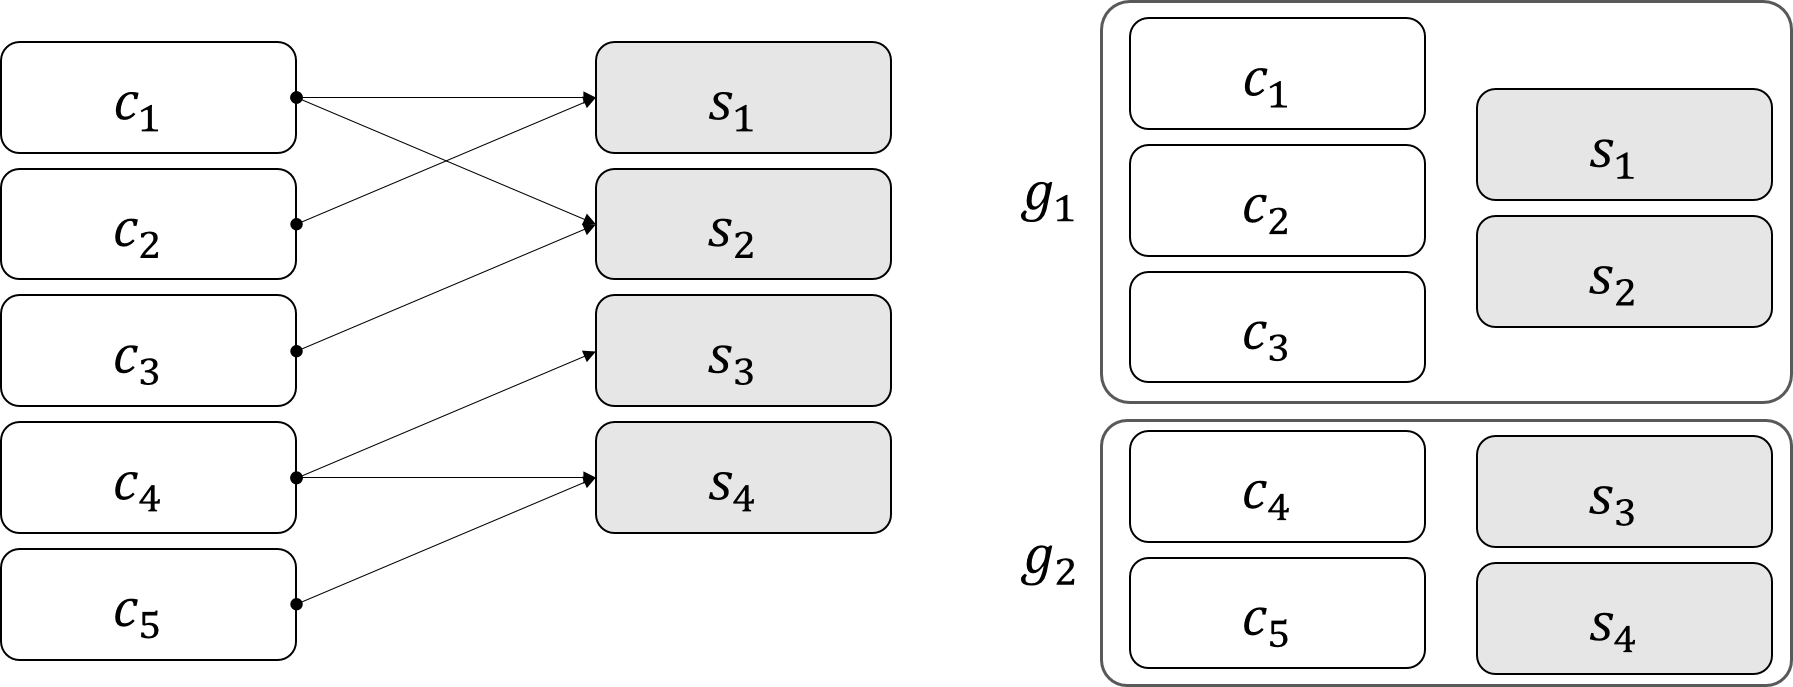
\includegraphics[width=0.95\linewidth]{images/correlationMap}
  \caption{(a)  Correlation map between rig space and skeleton space. (b) Body part grouping based on the correlation map}
  \label{fig:correlationMap}
\end{figure}
We formulate our inverse mapping as an optimization problem on the Lie algebra space. However, simultaneous optimization of all the parameters in the skeleton space and the rig space would not be efficient, because some of the rig parameters do not have any influence on some of the skeletons. Unfortunately, we do not have any prior information to identify these relationship. Therefore, we perform analysis with the following strategies:
\begin{itemize}
	\item Define the correlation map between the rig space parameter and the skeleton segment
	\item Divide the rig into several groups for which the rig operations are mutually independent 
\end{itemize}
After the rig analysis, we perform the optimization separately for each rig group. The rig analysis process is summarized in Algorithm 1.
\begin{algorithm}[ht]
    \caption{Rig Analysis}
    \SetKwInOut{Input}{Input}
    \SetKwInOut{Output}{Output}
    
    \Input{
	    Rig space parameters $\mathbf{c} = \left\{c_1, ..., c_m\right\}$,\newline
	    Individual skeletal segment parameters $\mathbf{s} = \left\{s_1, ..., s_k\right\}$
	    }
    \Output{
    Body part groups $G = \left\{g_1,g_2, ..., g_l\right\}$,\newline
    %Each group $g_i$ contains a set of corresponding rig parameters, skeleton parameters, \newline
    %Rig operations of $g_i$ in $G$ are mutually independent
    }
    $G \leftarrow \left\{g_1, ..., g_m\right\}$\;
    \For{each $c_i$ in $\mathbf{c}$}{
    		$g_i \leftarrow c_i$\;
    		$\check{\mathbf{c}}_i \leftarrow r \times randomSampling(c_i)$\;
    		$\check{\mathbf{p}}_\mathbf{s} \leftarrow poseMeasure(\check{\mathbf{c}}_i)$\;
    		
    		\For{each $s_j$ in $\mathbf{s}$}{
    			$\rho_{i,j} \leftarrow multipleCorrelation(\check{\mathbf{c}}_i, \check{\mathbf{p}}_{s_j})$\;
    			\If{$\rho_{i,j} \geq 0.5$}{
    				$g_i \leftarrow g_i \cup s_j$\;
    			}
    		}
    }
    \For{$\left\{g_i, g_j\right\}$ in $G$}{
	    \If{$\left\{g_i, g_j\right\}$ has same element}{
	    		merge $g_i$ and $g_j$\;
	    }
    }
   
   
    
%    create group $\hat{G} = \{\hat{g}_1, \dots, \hat{g}_m\}$\;
%    $\{\check{\mathbf{c}},\check{\mathbf{S}}\} \leftarrow r$ times of random value sampling per each $c$ in $C$\;
%	%\tcc*[h]{Random Value Sampling Process}\\
%	\For{ $c_i$ in $\mathbf{c}$, $s_j$ in $\mathbf{s}$ }{
%		%$k$ times of random value sampling for rig space parameter $c_i$ (range: $c_{min}<c_i<c_{max}$)\;
%		$\check{\mathbf{c}}_i \leftarrow \left\{ \check{c}^1_i, \dots, \check{c}^r_i \right\}$\;
%		$\check{\mathbf{s}}^j_{i} \leftarrow \left\{ \check{s}^{i,j}_0, \dots, \check{s}^{i,j}_k \right\}$\;
%		$\rho_{i,j} \leftarrow MultipleCorrelationCoefficient(\check{\mathbf{c}}_i, \check{\mathbf{s}}_i^j)$\;
%		%compute multiple correlation coefficient $\rho_{i,j}$ between $c_i$ and $s_j$ with sampled data list\;
%		\If {$\rho_{i,j} > 0.5$}{
%	    		union $g_i$ and $\{c_i, s_j\}$\;
%	    	}
%	}
%	%\tcc*[h]{Grouping Process}\\
%	\Repeat{no more groups have same element}{
%		\If{$g_i$ and $g_j$ have same element}{
%			union $g_i$ and $g_j$\;
%		}
%	}
	%\Return{$g = {g_1, ..., g_l}$}\;
\end{algorithm}
For a character composed of rig parameters $\mathbf{c}=\left\{ c_1, \dots, c_m \right\}$ and skeleton segments $\mathbf{s}=\left\{ s_1, \dots, s_k \right\}$,
we first define a \textit{correlation map} between $\mathbf{c}$ and $\mathbf{s}$.
Note that we only exploit relative transformation $A_{s_p,s_i}$ in the local coordinate system of $s_i$ about the parent skeletal segment $s_p$ during the rig analysis stage, to find \textit{direct} correlation between $c_j$ and $s_i$.
To construct a correspondence map without any prior information, we perform $r$ times of random value sampling per each $c_i$ in $\mathbf{c}$, and then measure the transformation changes of $\mathbf{s}$.
Then, we calculate multiple correlation coefficient $\rho_{i,j}$ between $c_i$ and $s_j$ that are sampled and measured data, respectively.
This represents correlation between $c_{i}$ and $s_{j}$  with a scalar value of range 0 to 1. Although the interpretation for the value of $\rho_{i,j}$ may depend on the context and purposes, we assume that $\rho_{i,j} < 0.5$ means that the two variables have no strong linear relationship\cite{mark2001practical}.

%Then, for each sample set for $c_i$, we calculate multiple correlation coefficient $\rho_{i,j}$ between $\check{\mathbf{c}}_i$ and $s_j$ using measured skeletal pose.
%$\check{\mathbf{c}}_i = \left \{ \check{c}^1_{i}, \check{c}^2_{i}, \dots, \check{c}^r_{i} \right \}$
%The sampled and measured data per each $c_i$ are represented as $\check{\mathbf{c}}_i = \left \{ \check{c}^1_{i}, \check{c}^2_{i}, \dots, \check{c}^r_{i} \right \}$.
%\def \cp {\check{\mathbf{p}}}
%\def \cc {\check{\mathbf{c}}}
%\begin{equation}
%	\begin{split}
%		\cc{}_i &= \left \{ \check{c}^1_{i}, \check{c}^2_{i}, \dots, \check{c}^r_{i} \right \}, \\
%		%\check{\mathbf{c}} &= \left \{ \check{c}^1_{1}, \check{c}^2_{1}, \dots, \check{c}^r_{m-1}, \check{c}^r_{m} \right \}, \\
%		\cp{}_i &= \left \{ \cp{}(\check{c}^1_i) \ldots \cp{}_i(\check{c}^r_i) \right \},
%	\end{split}
%\end{equation}
%
%Here, $\check{\mathbf{c}}_i$ is set of $r$ sampled rig parameters where $\check{c}^j_{i}$ denotes the $j$-th random value for $c_i$,
%and $\check{\mathbf{p}}_i$ is set of $r$ measured pose where $f(\check{c}^1_{i})$ denotes skeleton segments $\mathbf{s}$ given $\check{c}^j_{i}$.
%%$\check{\mathbf{s}}^j_{i} = \left\{ \check{s}^{i,j}_0, \dots,\check{s}^{i,j}_k \right\}$
%%$D_c$ and $D_s$ are the generated data lists by sampling.
%Next, we compute multiple correlation coefficient $\rho$ between
%$\check{\mathbf{c}}_i = \left\{ \check{c}^1_i, \dots, \check{c}^r_i \right\}$ which represents set of samples for $c_i$, and $\mathbf{s}_i = \left\{ \check{\mathbf{s}}_i^1 \ldots \check{\mathbf{s}}_i^r \right\}$.
%This returns 
%%$\check{\mathbf{s}}^j_i(n) = \left\{ \check{s}^{i,1}_j, \dots, \check{s}^{i,r}_j \right\}$.
%%$\check{c}_{i} \in r \times \mathbb{R}^1$ and $\check{s}_{j} \in r \times \mathbb{R}^6$ 
%This represents correlation between $c_{i}$ and $s_{j}$  with a scalar value of range 0 to 1. Although the interpretation for the value of $\rho_{i,j}$ may depend on the context and purposes, we assume that $\rho_{i,j} < 0.5$ means two variables have no strong linear relationship\cite{mark2001practical}.
%%In this way, we define the correlation map between $c$ and $s$ based on $\rho$.
%Figure~\ref{fig:correlationMap} (left) shows an example of the correlation map.
%If a $s_i$ is transformed when $c_j$ is modified, then the two parameters are connected.
%

The second goal of the rig analysis is to divide the rig into mutually independent groups.
We generate a set $\left\{g_1, g_2, \dots, g_m\right\}$ as the same size as $\mathbf{c}$ where each element of $g_i$ consists of $c_i$ and a set of skeletal segments $s_*$ whose $\rho_{i,*}$ is bigger than 0.5. Next, if any $\left\{g_i, g_j\right\}$ have at least one element in common, the two groups are merged. We merge repeatedly until there is no intersection among the 2 groups. The result is mutually independent rig groups $G$:
\begin{equation}
	G = \left \{ {g_{1}, g_{2}, ..., g_{l}} \right \},
\end{equation}
\begin{figure}[ht]
  \centering
  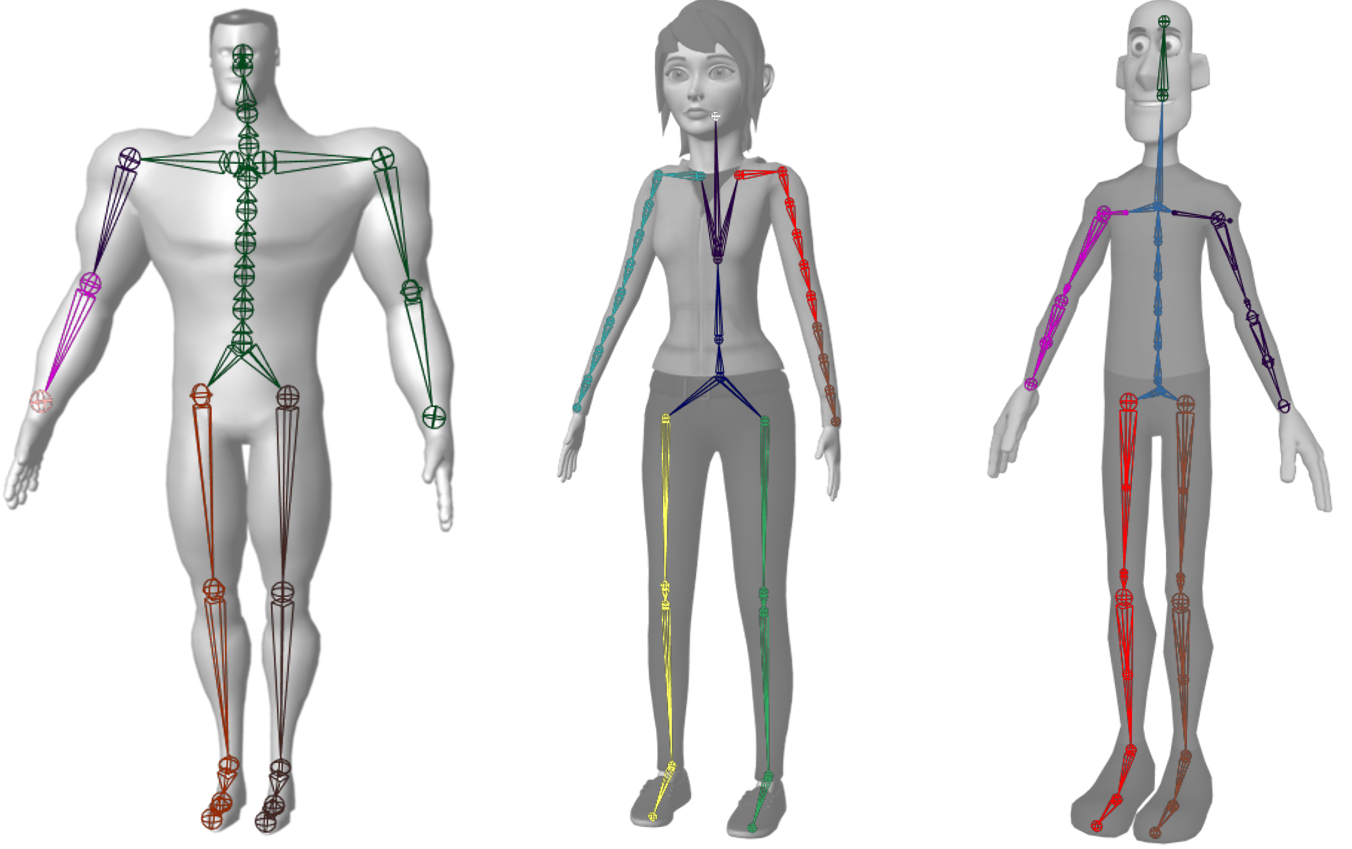
\includegraphics[width=0.85\linewidth]{images/bodyPartGrouping}
  \caption{Snapshots of various rig  grouping results}
  \label{fig:rigGroupingResult}
\end{figure}
Figure~\ref{fig:correlationMap}(right) shows an example of $G$. In our experimental results, we found that each $g_i$ is similar to the body part of a character, such as the limbs or the spine(Figure~\ref{fig:rigGroupingResult}). As our rig analysis process divides a complex non-linear full body problem into mutually independent body part sub-problems, our optimization can be performed close to linear relationship between the rig space and the skeleton space. 


%\newpage
\section{Spacetime Rig Optimization}
\label{section:spacetime}

%As we discussed in Section~\ref{sec:rig_opt}, our motion optimizaion in rig space is performed by minimizing the energy based on a skeletal motion distance.
%Although this results a successful inverse mapping, it is not practical enough to be used in production.
%In this section, we present constraints to get artist-friendly results.
%In this section, we present the details of spacetime optimization process which is based on a skeletal motion distance subject to the constraints derived from the %regularization of rig parameters, acceleration energy of rig parameters, relative body segment constraints, and rig parameter constraints.
In this section, we present the details of our spacetime optimization process discussed in Section~\ref{sec:rig_opt}.
The motion optimization in rig space is performed by minimizing the energy-based on a skeletal pose distance subject to the constraints derived from the regularization of rig parameters, acceleration energy of rig parameters, rig parameter constraint, and relative skeletal segment constraints.

%\begin{figure}[ht]
%  \centering
%  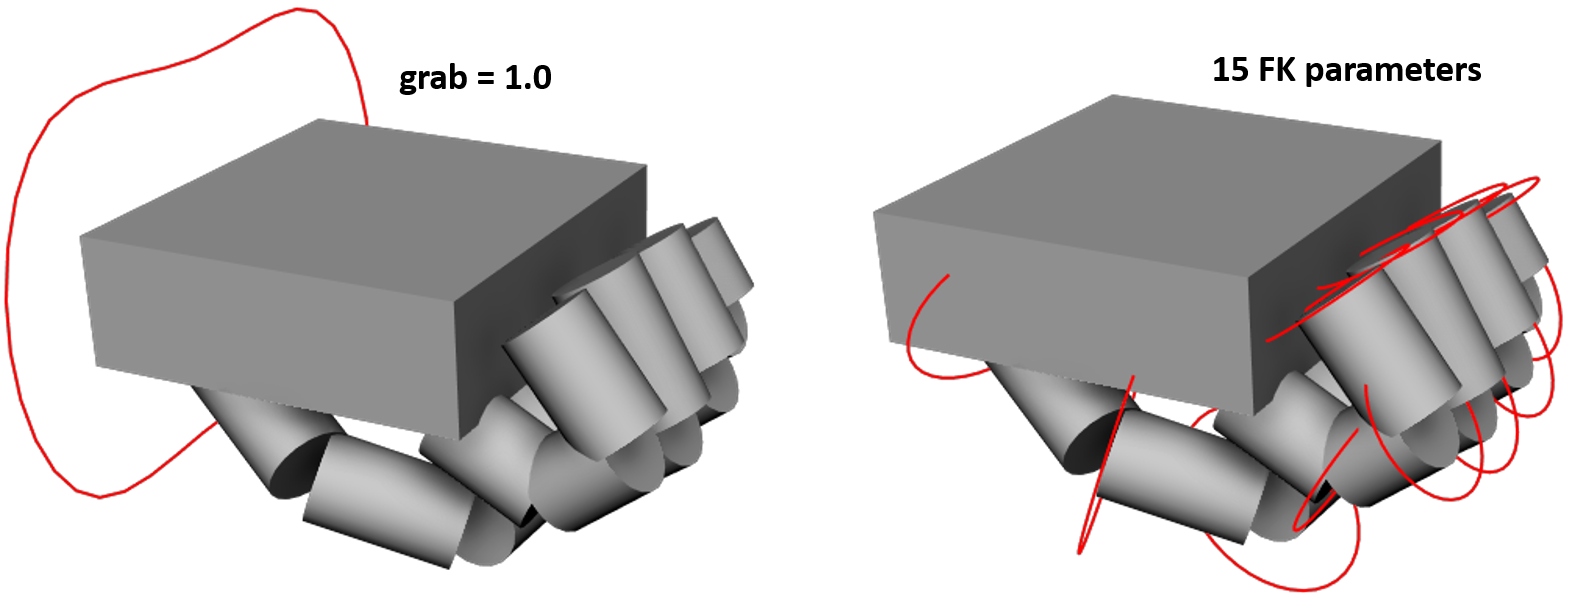
\includegraphics[width=3.0in]{images/handMultiSolution}
%  \caption{(a)Hand fist pose created by using one ‘grab’ parameter (b)Same pose created by using 15 FK parameters}
%  \label{fig:handRigExample}
%\end{figure}

%\begin{figure}[ht]
%  \centering
%  \begin{subfigure}[b]{0.20\textwidth}
%	  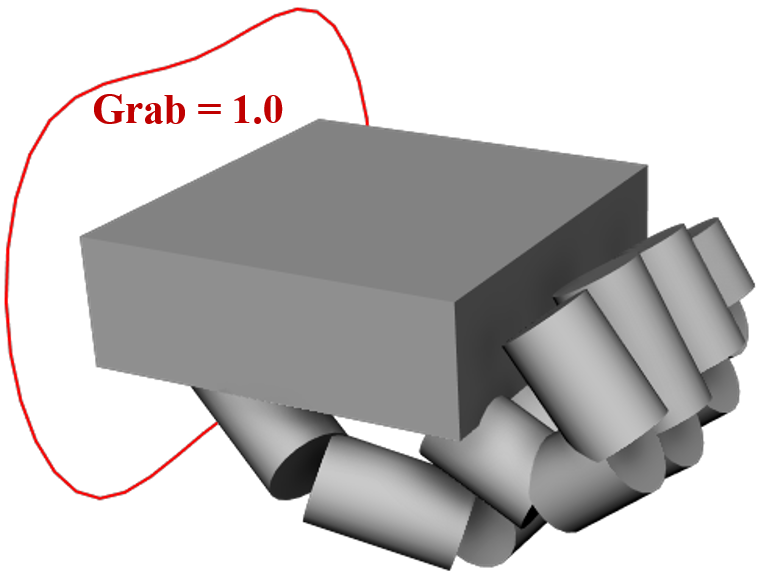
\includegraphics[width=3.0in]{images/grab}
%	  \caption{}
%	  \label{}
%  \end{subfigure}
%  \begin{subfigure}[b]{0.25\textwidth}
%	  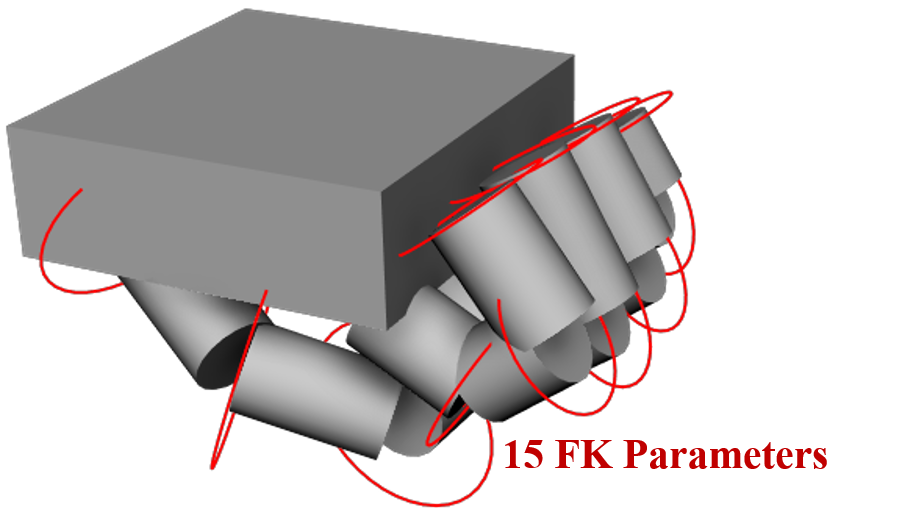
\includegraphics[width=3.0in]{images/fk15}
%	  \caption{}
%	  \label{}
%  \end{subfigure}
%  \caption{(a)Hand fist pose created by using one ‘grab’ parameter (b)Same pose created by using 15 FK parameters}
%  \label{fig:handRigExample}
%\end{figure}

\begin{figure}[!ht]
    \centering
    \begin{subfigure}[b]{0.2\textwidth}
        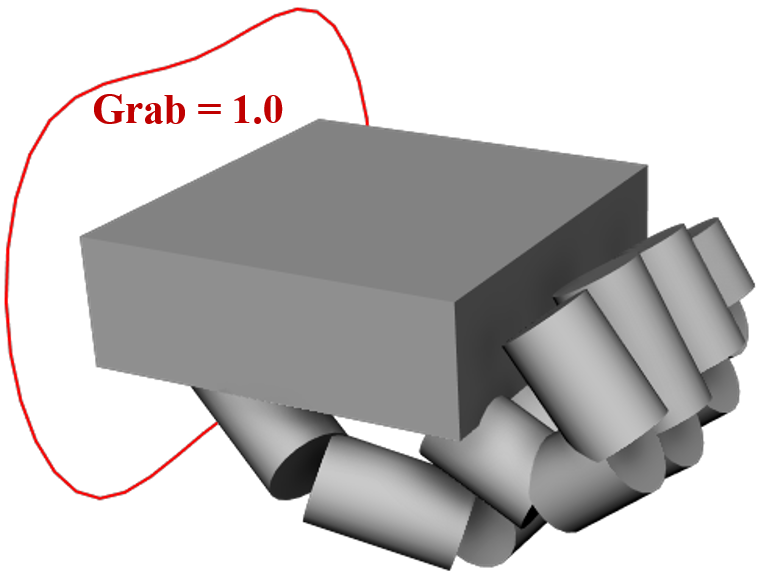
\includegraphics[width=\textwidth]{images/grab}
        \caption{}
        \label{}
    \end{subfigure}
    %add desired spacing between images, e. g. ~, \quad, \qquad, \hfill etc. 
      %(or a blank line to force the subfigure onto a new line)
    \begin{subfigure}[b]{0.23\textwidth}
        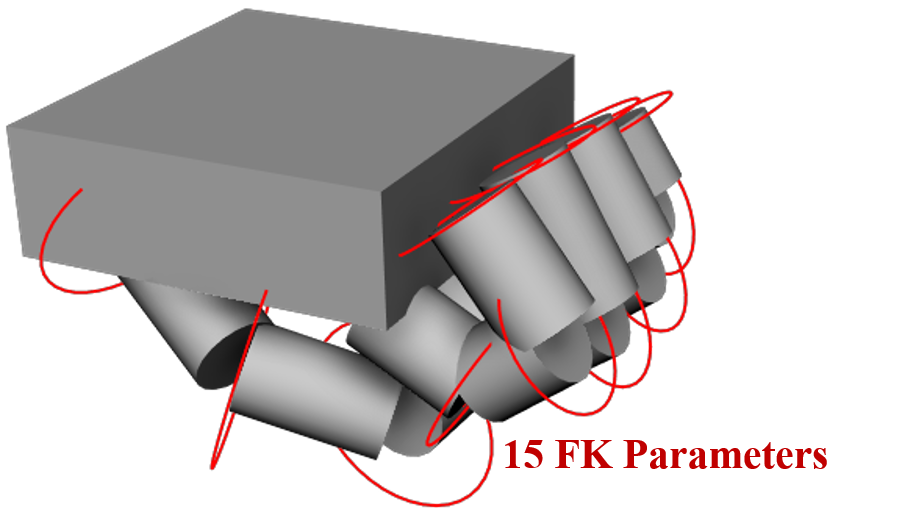
\includegraphics[width=\textwidth]{images/fk15}
        \caption{}
        \label{}
    \end{subfigure}
    
%    \begin{subfigure}[b]{0.45\textwidth}
%        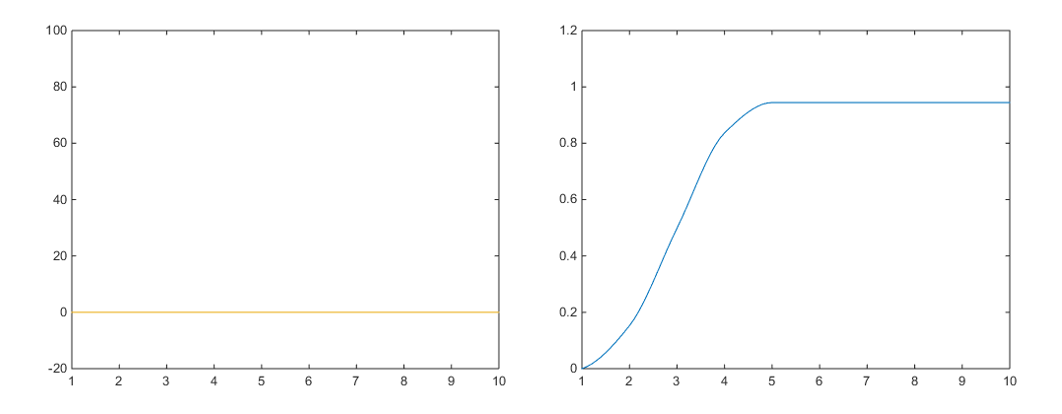
\includegraphics[width=\textwidth]{images/n1_big}
%        \caption{$\lambda = 1.0$}
%        \label{fig:reg_big}
%    \end{subfigure}
%    ~
%    \begin{subfigure}[b]{0.45\textwidth}
%        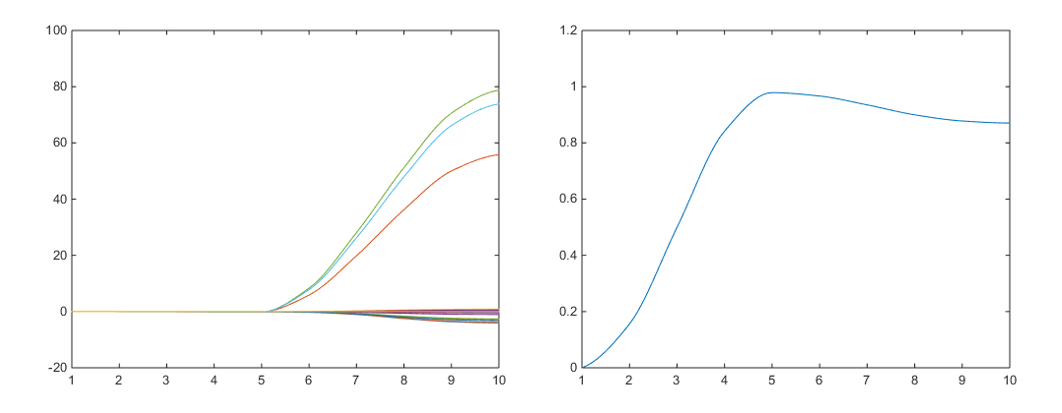
\includegraphics[width=\textwidth]{images/n1_small}
%        \caption{$\lambda = 0.0001$}
%        \label{fig:reg_small}
%    \end{subfigure}
    
    \caption{(a) Hand fist pose created by using one grab parameter (b) Same pose created by using 15 FK parameters
    }
    \label{fig:handRigExample}
\end{figure}


\textbf{Skeletal pose distance energy}
We illustrate the relationship between the skeletal pose $\mathbf{p}_i$ and its corresponding rig space parameter $\mathbf{c}_i$ in Section~\ref{sec:LigGroup}. Note that the solution of rig space parameter $\mathbf{c}_i$ for single pose $\mathbf{p}_i$ is not unique, in general. Figure~\ref{fig:handRigExample}(a) and (b) show that the same skeletal pose can be generated with different rig space parameters. In the animation production, the choice of rig space parameters is completely up to the preferences of the animator in such a case. Therefore, it is impossible to satisfy individual preference of the artist without any prior data. 
Instead, we define the optimality of the rig space parameters from the character rig functionality point of view. Riggers provide various functions to simplify the generation of complex motion with a small number of parameters\cite{orvalho2012facial}. In Figure~\ref{fig:handRigExample}, example (a) utilizes a custom parameter called \textit{grab} that activates on a single scalar value while example (b) relies on as many as 15 three dimensional \textit{FK} parameters. While the effects are same, the solution of example (a) is preferred over that of example (b) because it modifies fewer number of parameters. 
To reflect this, we choose the solution that involves a minimum number of parameters, when there are multiple solutions $\Delta{c(i)}$.
The energy term for the skeletal pose distance is represented as follows:

\begin{equation}
E_{p}(t) = \left \| \mathbf{J}(t)\Delta \mathbf{c}(t)-\Delta \mathfrak{p}(t) \right \|^{2}+\lambda \left | \Delta \mathbf{c}(t) \right |_1,
\end{equation}

where $\mathbf{J}$ is the Jacobian matrix of $\Delta \mathfrak{p}$ with respect to $\Delta\mathbf{c}$ at current time $t$, and $\lambda$ is the regularization weight parameter. The Jacobian matrix cannot be defined analytically because we do not assume any prior information about the exact function of each rig parameter. Therefore, we use approximate Jacobian obtained by finite differences of the current rig state. This process is known to be very slow\cite{hahn2012rig} because every rig parameter should be accessed to update the Jacobian. Fortunately, the Jacobian does not have to be recomputed in every iteration because when the rig skeletal pose approaches to the target pose, the Jacobian remains alomost the same. Our experiments show that the fine tuning of the pose requires more than 60\% of the computation time. Therefore, we reuse the same Jacobian from the previous iteration when the current pose distance is smaller than a threhshold $\eta$. Moreover, we already reduced the number of rig parameters in the rig analysis stage, thus we could enhance the performance of the Jacobian computation. The threshold $\eta$ is user parameter that depends on the number of skeletal segments and the global scale of the character. In our experiment, $\eta = 0.1$ showed reasonable results.
%We locally compute Jacobian matrix $\mathbf{J}$ at the current state and find $\Delta \mathbf{c}^*(t)$ to reach the target pose $\bar{\mathfrak{p}}(t)$ by performing the local linear approximation on the Lie algebra vector space. 
%\textbf{For faster computation time, we updated the $\mathbf{J}$ until the pose distance is under certain threshold, and used the same one until it converge.}

Note that we performed the L1 regularization on $\Delta{c}$. The L1 regularization favors a sparse solution of rig parameters and force the small weight parameters converge to 0. This allows to provide the animator with the minimum number of resulting parameters to deal with, for the creation of animation.
Our solution also satisfies the artist's preference toward sparse parameters in generating motions\cite{seol2011artist}. Although the optimal regularization weight $\lambda$ can be estimated through the cross-validation after the optimization, the value of $0.001$ achieved reasonable regularization for various rigs in our experiments.

\textbf{Acceleration energy}
Since we optimize rig space parameters for each pose, popping artifact may occur. To address this, we minimize the acceleration energy at time $t$, so that the rig space parameters change smoothly across adjacent frames:
\begin{equation}
E_{a}(t) = \frac{1}{2}\left \| \Delta C(t-1)-2\Delta C(t)+\Delta C(t+1) \right \|^{2}, \\
\end{equation}

\subsection{Constraints}

\textbf{Rig parameter constraint}
Although we provide the optimal solution from a rig functionality point of view, the artist may prefer a different solution depending on the situation. We introduce a rig parameter constraint $K_{anim}$ to incorporate the artist's preference in the optimization process. The rig parameter constraint provided by the artist is calculated as:

\begin{equation}
K_{anim} (t) = \mathbf{K}_{anim}(t) \Delta C(t) - \mathbf{h}_{anim},
\end{equation}

where $\mathbf{K}_{anim}$ is the system constraint matrix (See Appendix A for details), and $\mathbf{h}_{anim}$ is the constraint vector that pushes the rig parameter toward the value designated by the artist.

\textbf{Relative skeletal segment constraints}
Self-penetration is one of the frequently occurr errors that the artist has to fix after the mapping to the rig space. The self-penetration occurs in the vertex level and the mesh level collision detection is not considered in this paper. Instead, we let the artist specify relative distance constraints between the skeletal segments. The relative distance constraint is represented as relative transformations between the two skeletal segments. Therefore, the relative skeletal segment constraint $K_{rel}$ at time $t$ is defined as follows:

\begin{equation}
K_{rel} (t) = \mathbf{K}_{rel}(t) \Delta C(t) - \mathbf{o}_{rel},
\end{equation}

where $\mathbf{K}_{rel}$ is the Jacobian matrix that represents how the relative transformation between the two body segments are changed by rig space parameter $\Delta C(t)$. $\mathbf{o}_{rel}$ represents the pose distance from current rig segments pose to desired pose given by the artist. Although our optimization is performed separately for each rig group, the relative distance constraint can be applied to any skeletal segment. For example, even if the arm and the spine of a human character is divided into two different groups, the constraint can be applied to prevent the two segments from colliding with each other.

%\textbf{Constraint energy}
%
%\begin{equation}
%\begin{split}
%E_{k} = \frac{1}{2} \Delta C^{T}\mathbf{K}^{T}\mathbf{W}\mathbf{K}\Delta C - \mathbf{k}^{T}\mathbf{W}\mathbf{k} +
%\frac{1}{2}\mathbf{k}^{T}\mathbf{W}\mathbf{k}
%\end{split}
%\end{equation}
%where $W$ is weight matrix that the purpose is assigning different weight to each constraint.

\subsection{Iterative optimization} \label{objectiveFunction}
We defined the relative skeletal segment constraint as a soft constraint, and the rig parameter constraint as a hard constriant.
Denoting the soft constraint as $E_s$ and the hard constraint as $E_h$, the objective function can be represented as follows:

\newcommand{\argmin}{\operatornamewithlimits{argmin}}

\begin{equation}
\argmin_{\Delta{\mathbf{c}(t)}}{\sum_t^n \left( {E_p(t) + w_aE_a(t)+E_s(t)+ \mathbf{z}^T E_h}\right)},
\label{eq:objectiveFtn}
\end{equation}

where $n$ indicates the number of frames, $w_a$ is the weight for the acceleration energy, and $\mathbf{z}$ denotes the Lagrange multipliers. $E_a$ at the first and the last frame is zero. Eq.~\ref{eq:objectiveFtn} can be rewritten in a matrix form as follows:
\begin{equation}
\begin{split}
\begin{bmatrix}
\boldsymbol{J}^T\boldsymbol{J}+w_a\boldsymbol{A}^T\boldsymbol{A}+\boldsymbol{K}_s^T\boldsymbol{W}\boldsymbol{K}_s+\boldsymbol{L} & \boldsymbol{K}_h^T\\ 
\boldsymbol{K}_h & 0 
\end{bmatrix}
\begin{bmatrix}
\Delta\boldsymbol{C}\\ 
\boldsymbol{Z}
\end{bmatrix}\\
=
\begin{bmatrix}
\boldsymbol{J}^T\Delta\boldsymbol{S} + \boldsymbol{K}_s^T\boldsymbol{W}\boldsymbol{k}_s\\ 
\boldsymbol{H}
\end{bmatrix},
\end{split}
\end{equation}

where $\boldsymbol{J}$, $\boldsymbol{K_s}$, $\boldsymbol{K_h}$ are diagonalized block matrices in time t of $\mathbf{J}$, $\mathbf{K_{anim}}$, $\mathbf{K_{rel}}$, respectively, $\Delta\boldsymbol{C}$, $\boldsymbol{Z}$, $\Delta\boldsymbol{S}$ and $\Delta\boldsymbol{H}$ are concatenated vector in time t of $\Delta\mathbf{c}$, $\Delta\mathbf{z}$, $\Delta\mathbf{s}$ and $\Delta\mathbf{h}$ respectively, and $\boldsymbol{W}$ is weight matrix for $\boldsymbol{K_s}$. $\boldsymbol{L}$ and $\boldsymbol{A}$ are the regularization matrix and the acceleration energy matrix, respectively\cite{ho2010spatial}.(See Appendix A for full details)
%$\boldsymbol{L}$ is regularization constraint matrix, and $\boldsymbol{A}$ is accereleration energy matrix where each is explained in Appendix.
The optimization terminates if it reaches the maximum iteration number $max_i$ or the magnitude difference of the rig space parameter $||\Delta c(t)||^2$ between the iteration steps is below a certain threshold $\epsilon$. 

%Since the each body segment group is independent, the order of optimization each group is irrelevant. 

%Our optimization is performed iteratively at every timestep(frame) $t$.

%Here, we set the user parameter $(max_i, \epsilon)$ as $(100, 10^{-100})$.
%Note our results are optimized in order of hierarchy of skeleton structure.
%\newpage
\section{Results}

\newcolumntype{C}[1]{>{\centering\let\newline\\\arraybackslash\hspace{0pt}}m{#1}}

\begin{table*}[]
\centering
\label{my-label}
\begin{tabular}{|c|C{0.8cm}|C{0.8cm}|C{0.8cm}|C{0.8cm}|C{0.8cm}|C{0.8cm}|C{0.8cm}|C{0.8cm}|C{0.8cm}|C{0.8cm}|C{0.8cm}|C{0.8cm}|}
\hline
\multirow{2}{*}{Motion} & \multicolumn{2}{c|}{Ours} & \multicolumn{2}{c|}{Joint Position} & \multicolumn{2}{c|}{Yaw Pitch Roll} & \multicolumn{2}{c|}{Quaternion} & \multicolumn{2}{c|}{Matrix Elements} & \multicolumn{2}{c|}{$\mathfrak{se}3$ only} \\ \cline{2-13} 
                        &$t$ &$e$  &$t$  &$e$  &$t$  &$e$  &$t$  &$e$  &$t$  &$e$  &$t$  &$e$  \\ \hline
Dunk(90 frames)         &3.18 &9.88   &2.14 &40.71    &6.544 &55.38  &3.88 &10.03  &4.01 &11.15    &3.04 &12.73 \\ \hline
Walk(397 frames)        &1.78 &4.48   &1.60 &13.48    &11.70 &36.60     &4.55 &21.35  &2.63 &15.26    &1.72 &4.96 \\ \hline
Jump*(90 frames)     &3.52 &20.30   &3.67 &56.41   &8.17 &51.36  &4.20 &28.61  &2.32 &26.18       &4.33 &41.73 \\ \hline
Average			     &2.83 &11.55   &2.47 &36.87   &8.80 &47.78      &4.21 &20.00  &2.99 &17.53   &3.03 &19.81 \\ \hline
\end{tabular}
\caption{Average error $e$ and comutation time $t$ required for the mapping of three different target motions using various skeletal representations.
The character has 85 rig space parameters and 35 skeletal segments, and we limit the maximum iteration to 100.
$e$ is calculated in the proposed skeletal representation, and the unit of $t$ is $sec/frame$.
*Jump motion includes stylized squash-and-stretch motion as shown in Figure~\ref{fig:squashResult}.
}
\label{table:poseRepresentEvaluation}
\end{table*}

We first compare the proposed skeletal pose representation with other representations. Next, we present several examples to demonstrate how our optimization resolves ambiguity caused by the inverse mapping and modifies the results corresponding to the input by the artist. We applied our method to the animation production pipeline to verify that our method can actually improve the productivity in the creation and editing of character animation in the real production environment.

To verify the versatility of our motion mapping, we performed the experiments with various characters.
Both motion capture data and keyframed animations were used as retargeting sources, and all the motions were adjusted to be 30 frames per second. To test our method in the Autodesk Maya 2016 environment, we implemented the system as a plug-in with Maya python script. A 3.40GHz Intel i7-3770 processor with 8GB memory is utilized for all of the experiments.

\textbf{Pose representation evaluation}
We performed the same rig space motion mapping with different skeletal representations to show that the proposed skeletal representation outperforms the other representations in terms of efficiency and correctness. We measured the computation time and the error of the skeleton at joint positions, joint angles(Yaw-Pitch-Roll), Quaternion, elements of a transformation matrix, hierarchy only representation of Lie group, and our representation. Table~\ref{table:poseRepresentEvaluation} shows the results. The result verfies that our pose representation provides an efficient and precise solution compared to other pose representations.

\textbf{Ambiguous parameter optimization}
The rigs for the hand usually composed of several user defined parameters to create complex fingers motions. Parameter grab(Figure~\ref{fig:handRigExample}) is an examples of the user defined parameters, which is designed to activate all of the finger motions simultaneously. However, FK parameters for each finger can also be useful to generate individual finger motion. In this ambiguous case, we provide the optimial solution depending on the given tasks, which exploits the minimum number of the rig space parameters. Figure~\ref{fig:handExample} illustrates the tasks with different goals. The desired action of the rig space parameters in this example would be to activate one grab parameter to create the fist pose, followed by activating three FK parameters associated with the index finger to create a pointing pose. Figure~\ref{fig:reg} shows the graphs generated by applying our sparse solution with L1 regularization and with conventional L2 regularization. The comparison of the graphs verifies that our L1 regularization method provides a desired sparse solution for each tasks.

\begin{figure}[!ht]
  \centering
  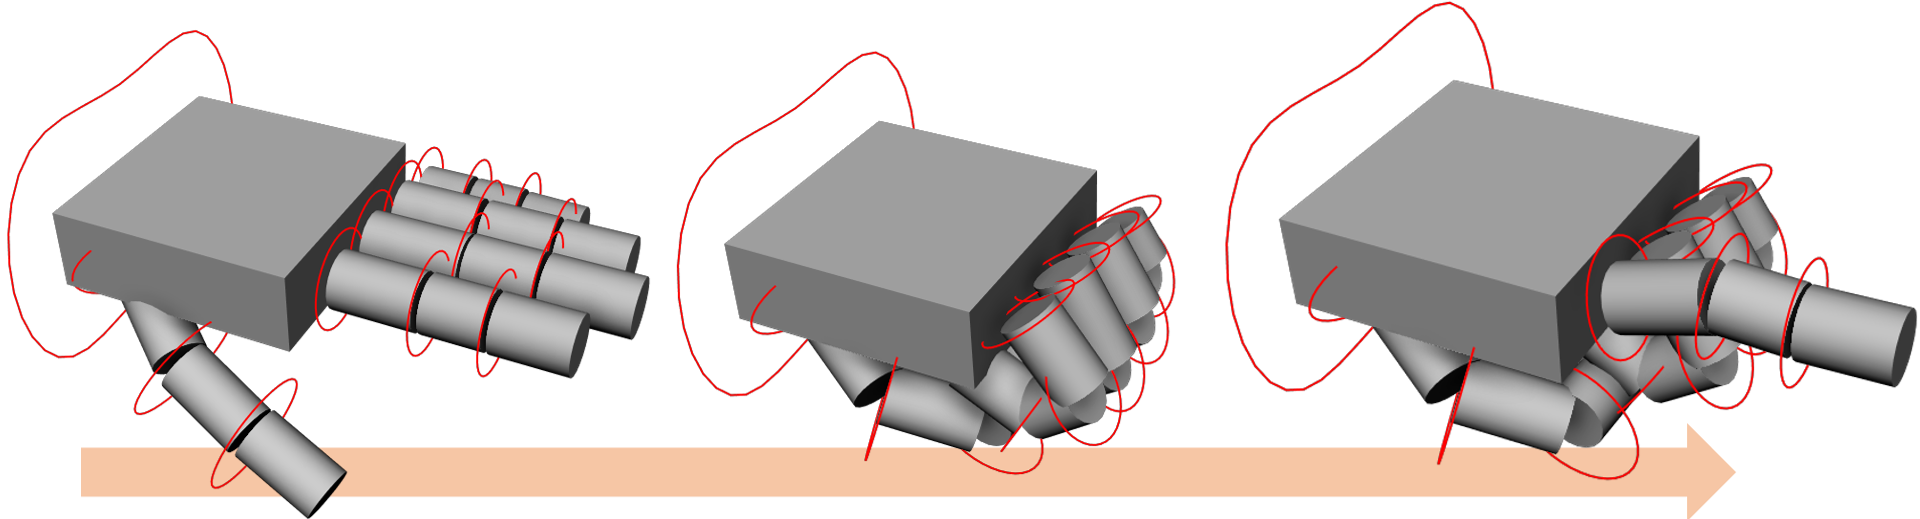
\includegraphics[width=3.0in]{images/handExample}
  \caption{Optimization results for the hand rig. The given motion is a sequence of the neutral, fist, and pointing hand pose.}
  \label{fig:handExample}
\end{figure}

\begin{figure}[!ht]
    \centering
    \begin{subfigure}[b]{0.48\textwidth}
        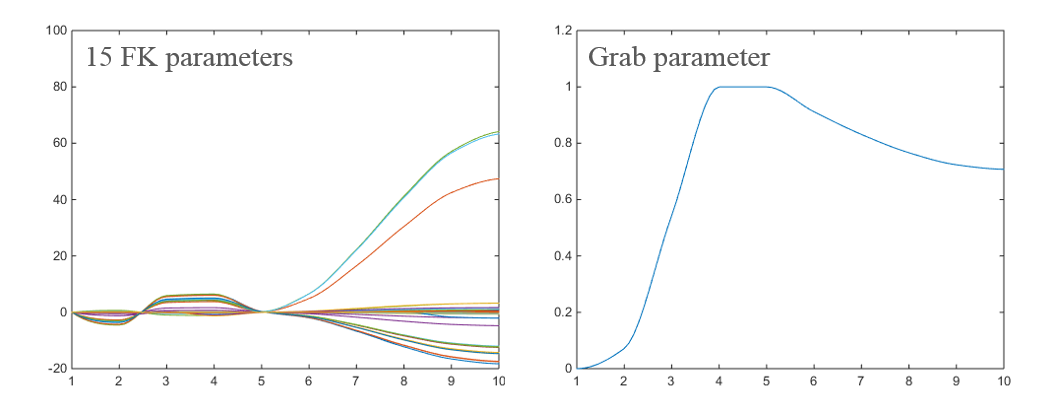
\includegraphics[width=\textwidth]{images/ls}
        \caption{L2 regularization}
        \label{fig:ls}
    \end{subfigure}
    %add desired spacing between images, e. g. ~, \quad, \qquad, \hfill etc. 
      %(or a blank line to force the subfigure onto a new line)
    \begin{subfigure}[b]{0.48\textwidth}
        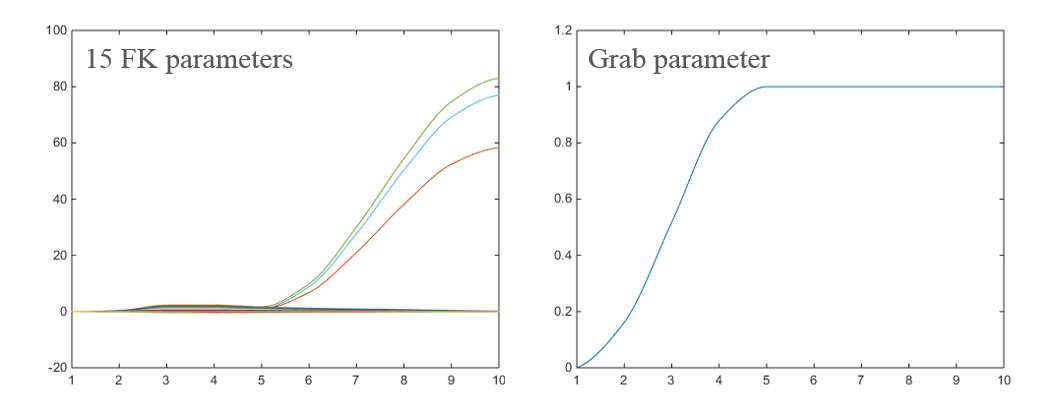
\includegraphics[width=\textwidth]{images/n1_good}
        \caption{L1 regularization ($\lambda = 0.001$)}
        \label{fig:reg_opt}
    \end{subfigure}
    
%    \begin{subfigure}[b]{0.45\textwidth}
%        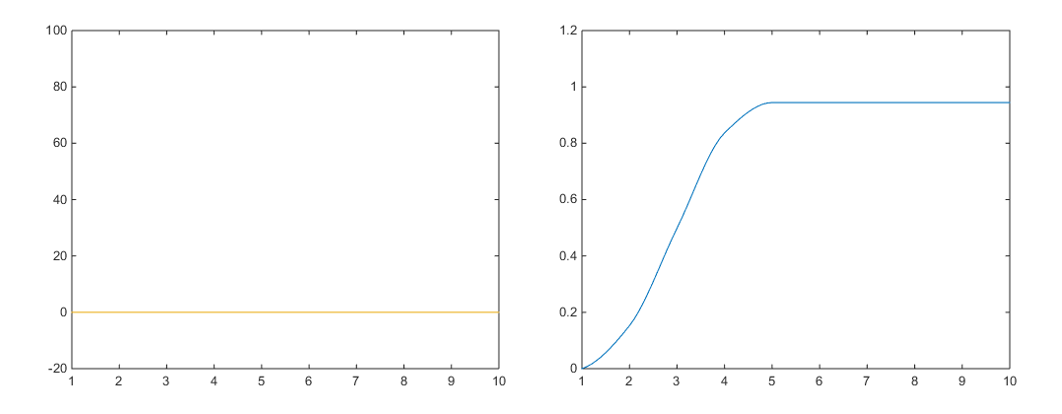
\includegraphics[width=\textwidth]{images/n1_big}
%        \caption{$\lambda = 1.0$}
%        \label{fig:reg_big}
%    \end{subfigure}
%    ~
%    \begin{subfigure}[b]{0.45\textwidth}
%        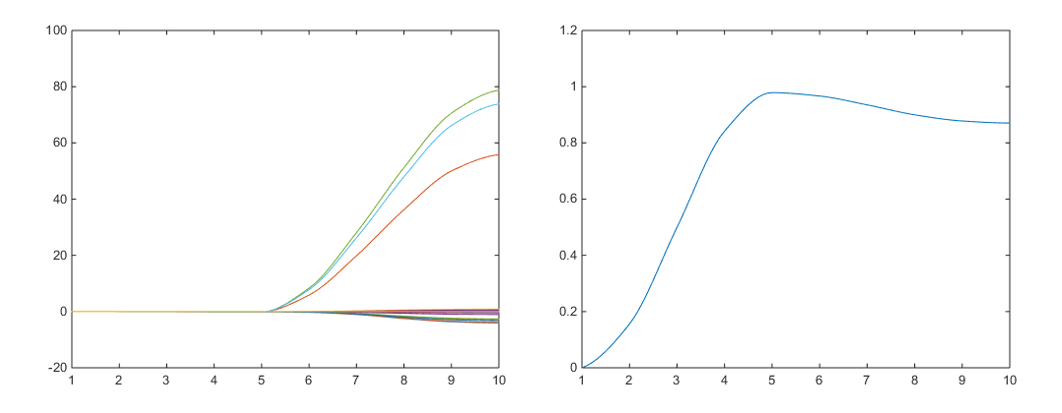
\includegraphics[width=\textwidth]{images/n1_small}
%        \caption{$\lambda = 0.0001$}
%        \label{fig:reg_small}
%    \end{subfigure}
    
    \caption{Comparison between optimization results of Figure~\ref{fig:handExample}.
    (a) FK parameters associated with all the fingers and grab parameter are used to generate pointing hand pose.
    (b) FK parameters of the index finger and grab parameter are used to generate the pointing hand pose.
    }
    \label{fig:reg}
\end{figure}

%\begin{figure*}[!ht]
%  \centering
%  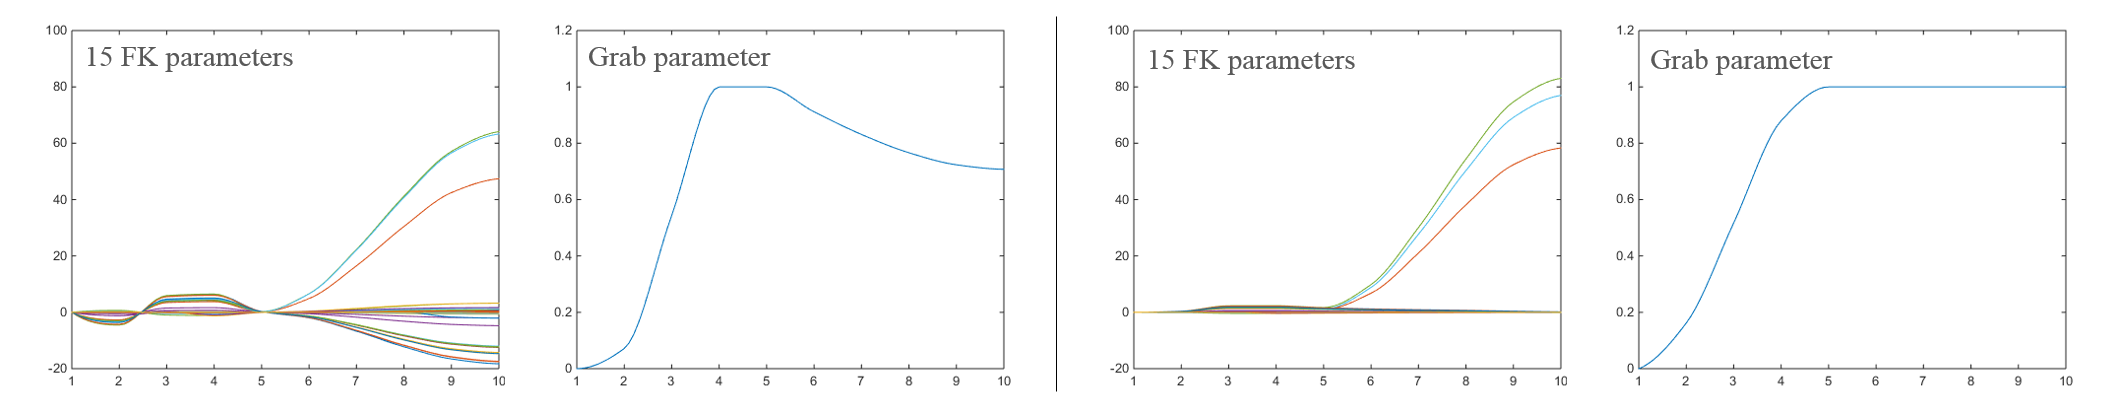
\includegraphics[width=0.95\textwidth]{images/reg}
%  \caption{Comparison between optimization results of Figure~\ref{fig:handExample}. ($\lambda = 0.001$) (left) L1 regularization (right) L2 regularization}
%  \label{fig:reg}
%\end{figure*}

%
%\begin{table}[ht]
%  \centering  
%  \begin{tabular}{|b|b b b|}
%    \hline
%     & Pose(a) & Pose(b) & Pose(c)\\
%    \hline
%    grab     & 1 & 1 & 0 \\
%    fingerFk & 0 & 6 & 15 \\
%    N(R)     & 1 & 7 & 15 \\
%    \hline
%  \end{tabular}
%  \caption{The number of activated rig parameters for various hand poses.}
%\end{table}

\textbf{Mapping results for various characters}
We applied the motion mapping to vaious target character rigs. Three different characters, which are rigged with FK only, FK+IK, and FK+IK+user defined parameters, respectively, are prepared for this purpose. Our method successfully maps the motion to various types of the rig space parameters as shown in Figure~\ref{fig:variousResult}. 
We also applied our method to a nonhuman character as shown in Figure~\ref{fig:dogResult}.
Figure~\ref{fig:squashResult} shows a result of our mapping of a stylized motion. As long as the rig space parameters can represent squash-and-stretches of the body parts, exaggerated source motion can be retargeted to a target character without any special treatment.
Although the pose representation with Lie group \SE{} is designed to work with rigid body motions, our method retargets stylized motion successfully, because the squash-and-strech motion can be represented by the translation of the skeletal segments.
This provides animation with great advantages of reusing high quality keyframed motions created by artists for different characters.

\begin{figure}[ht]
  \centering
  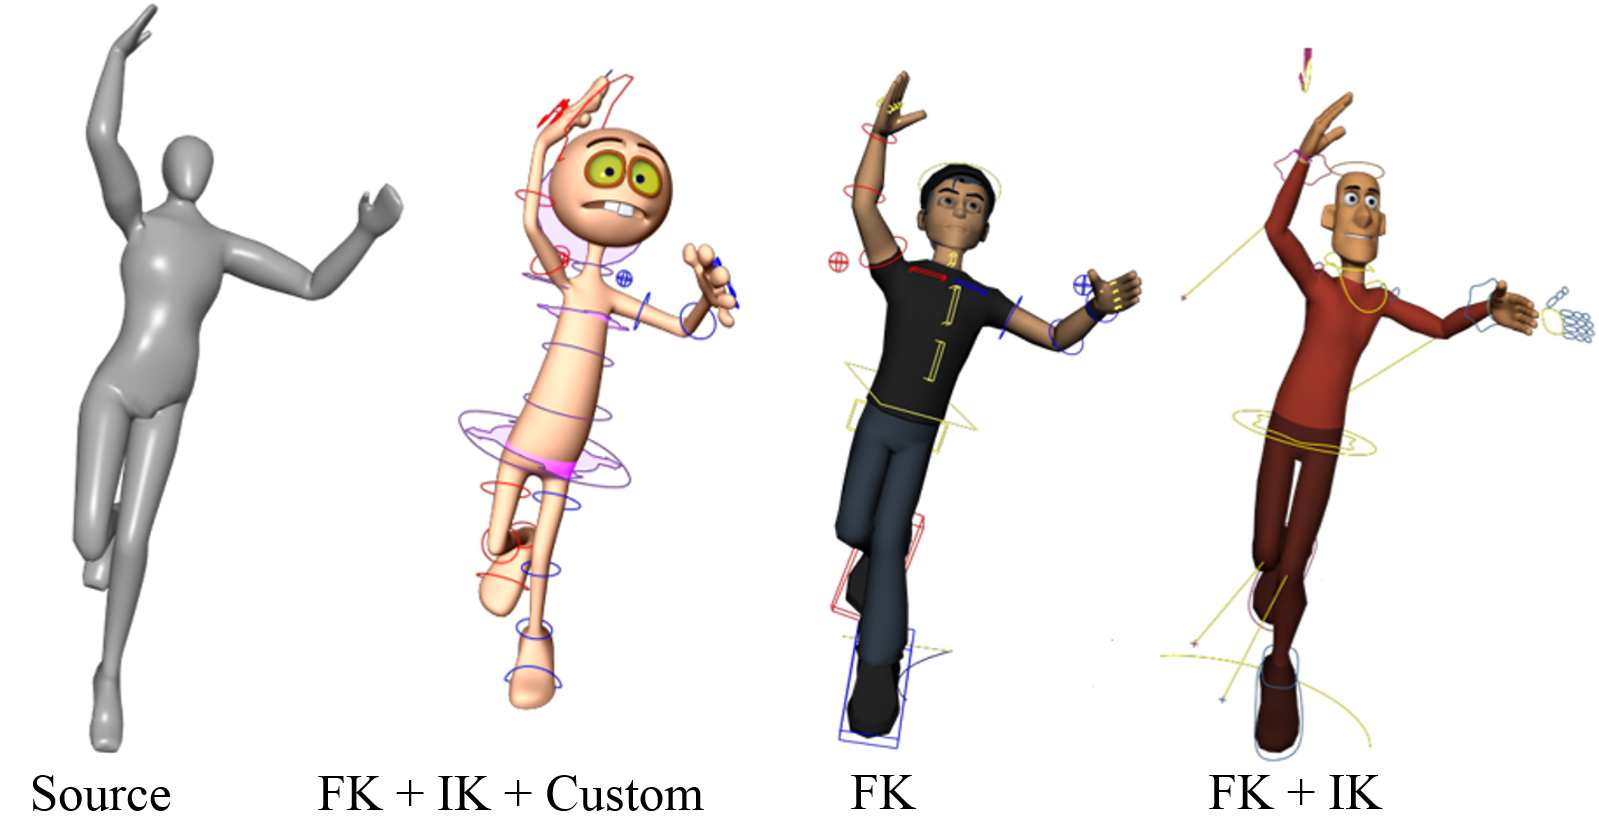
\includegraphics[width=1.0\linewidth]{images/various}
  \caption{Motion mapping results for three different characters.}
  \label{fig:variousResult}
\end{figure}

\begin{figure}[ht]
  \centering
  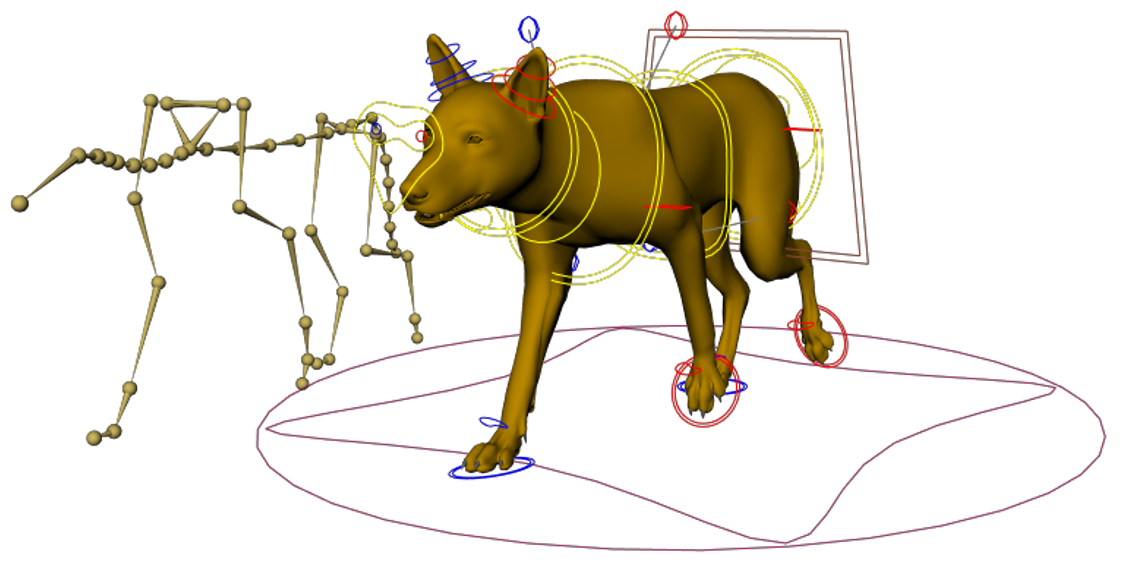
\includegraphics[width=.9\linewidth]{images/dogResult}
  \caption{Motion mapping results on quadruped character. }
  \label{fig:dogResult}
\end{figure}

\begin{figure}[ht]
  \centering
  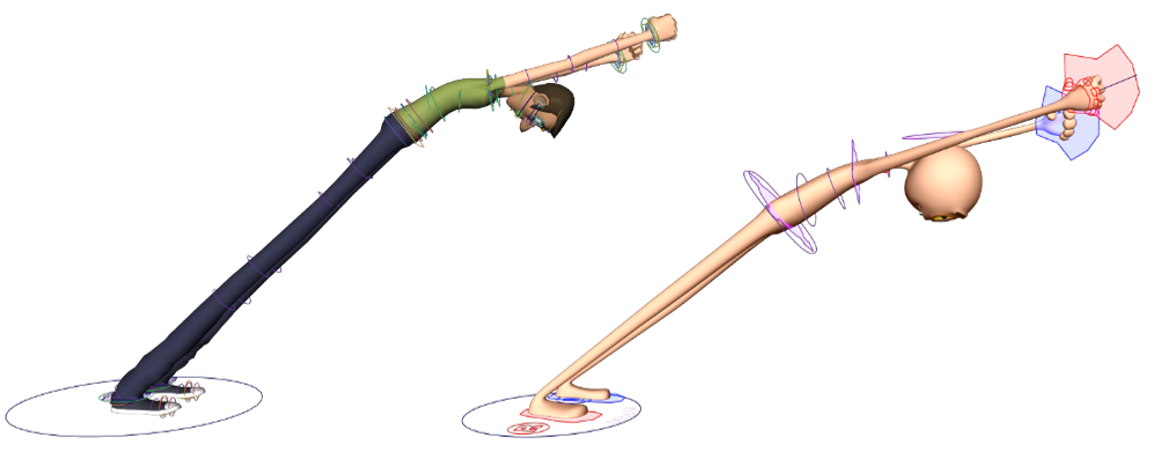
\includegraphics[width=.9\linewidth]{images/squashResult}
  \caption{Motion mapping result of stylized squash-and-stretch motion. }
  \label{fig:squashResult}
\end{figure}


\textbf{Editable optimization}
We provide the artist with editable optimization that is based on the relative skeletal segment constraint and the rig parameter constraint. Figure~\ref{fig:selfPenetration} shows a result of applying the relative skeletal constraint. Self-penetration is one of the most frequently occurring problems after a retargeting process, in general. Instead of performing the heavy mesh-level collision computation, we simply alleviate the problem with the use of relative constraints between the skeletal segments. 

\begin{figure}[ht]
  \centering
  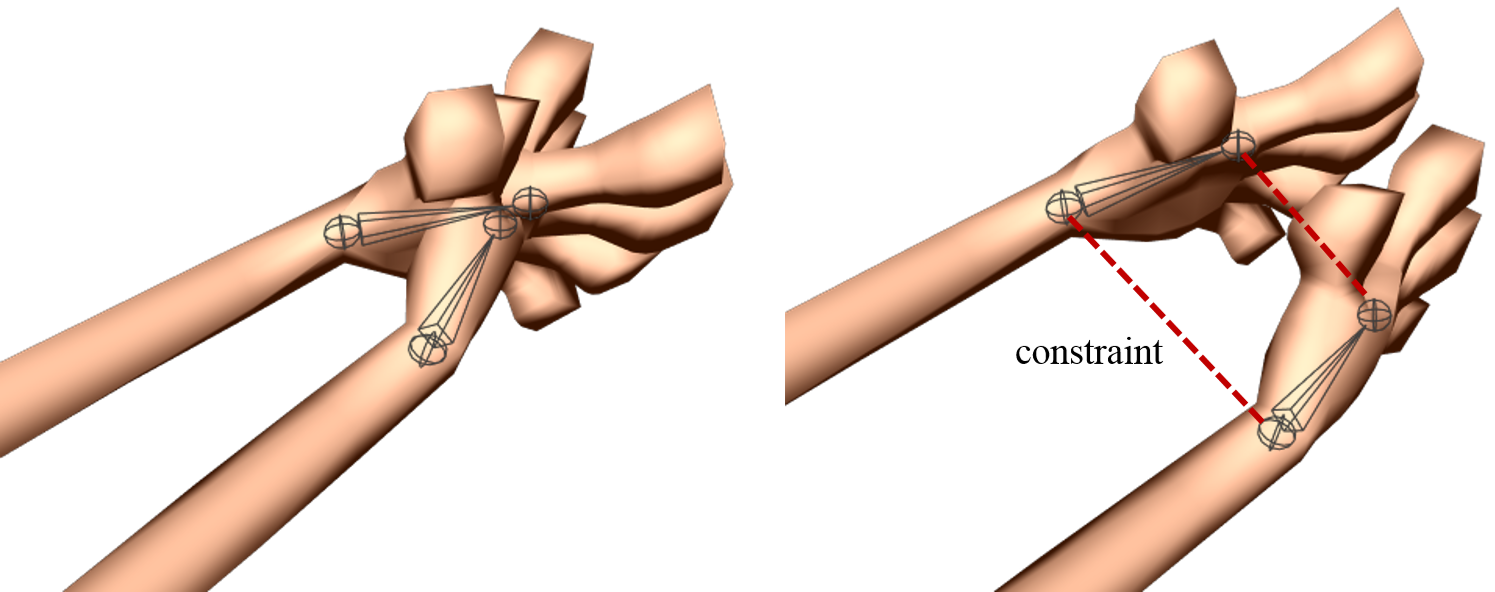
\includegraphics[width=.9\linewidth]{images/selfPenetration}
  \caption{(left) Self-penetration error after the initial optimization. (right) After the application of relative skeletal segment constraint given by artist.}
  \label{fig:selfPenetration}
\end{figure}

\textbf{Production pipeline evaluation}
Our method is suitable for the production pipeline, because the results produced by the rig space retargeting are something that artists would expect.
The subsequent editing process can be performed seamlessly.
To verify this, we applied our method to an animation project that exploits motion capture data as shown in Figure~\ref{fig:productionPipeline} which includes dynamic motions such as sword fighting and attacking of the dog.
For comparison, we additionaly measured working time required by 2 different methods to create the same animation: using keyframing and motion capture editing with commercial software, Autodesk MotionBuilder.
We performed the test with three different artists: one has 3 years of experiences, and the other two have 7 monthes of experiences.
As shown in Table~\ref{table:editing_evaluation}, our method required less time than keyframing or using commercial software. This verifies that our method can increase  efficiency in production.
Since artists are trained with using rigs in the existing animation pipeline, they also preferred our method that allows them to use the character rigs to edit the motion.
%All the animations were generated by three artists, one with 3 years experiences and the other two with 7 monthes of experiences.

%create a keyframe animation similiar to the motion capture scene. Then, we applied our method to the given motion capture data and the character rigs and presented to the artists for editing. Then, we measured the working time for both of the keyframing and the motion capture editing using our method.
%In addition, we measure the working time of motion capture editing with commercial software, Autodesk MotionBuilder$\textregistered$. 
%As shown in Table~\ref{table:editing_evaluation}, our method required less time than keyframing.


%\begin{table}[]
%\centering
%
%\begin{tabular}{c|c|c}
%\hline
%Artists                                                                                             & Method      & Working Time \\ \hline
%\multirow{3}{*}{\begin{tabular}[c]{@{}c@{}}One with 3-years of experience\\ \\ Two with 7-months of experience\end{tabular}} & Keyframing  & 10.7 Days    \\ \cline{2-3} 
%                                                                                                    & Mocap + MB   & 5 Days       \\ \cline{2-3} 
%                                                                                                    & Mocap + Ours & 3 Days       \\ \hline
%\end{tabular}
%\caption{Evaluation of our method to compared with keyframing and commercial software in the production pipeline environment.}
%\label{table:editing_evaluation}
%\end{table}
\begin{table}[!ht]
\centering
\begin{tabular}{ | c | c | }
  \hline
  Method & Average Working Time \\ \hline
  Mocap + Our Method & 3 Days \\ 
  Mocap + Commercial Software & 5 Days \\
  Keyframing & 10.7 Days \\
  \hline
\end{tabular}
\caption{Evaluation of our method compared with keyframing and using commercial software in the production pipeline environment. The result animations have 1140 frames.}
\label{table:editing_evaluation}
\end{table}

%\textbf{
%They create the dynamic motion of character efficiently from the motion capture editing with our method.
%Our method also required less amount of time to achieve the animation goal compared to the use of commercial software, because the artists are not expert with the software, and they prefer to use the character rigs to edit the motion because they already trained with the rigs in the exisiting animation pipeline. 
%}

\begin{figure}[!ht]
  \centering
  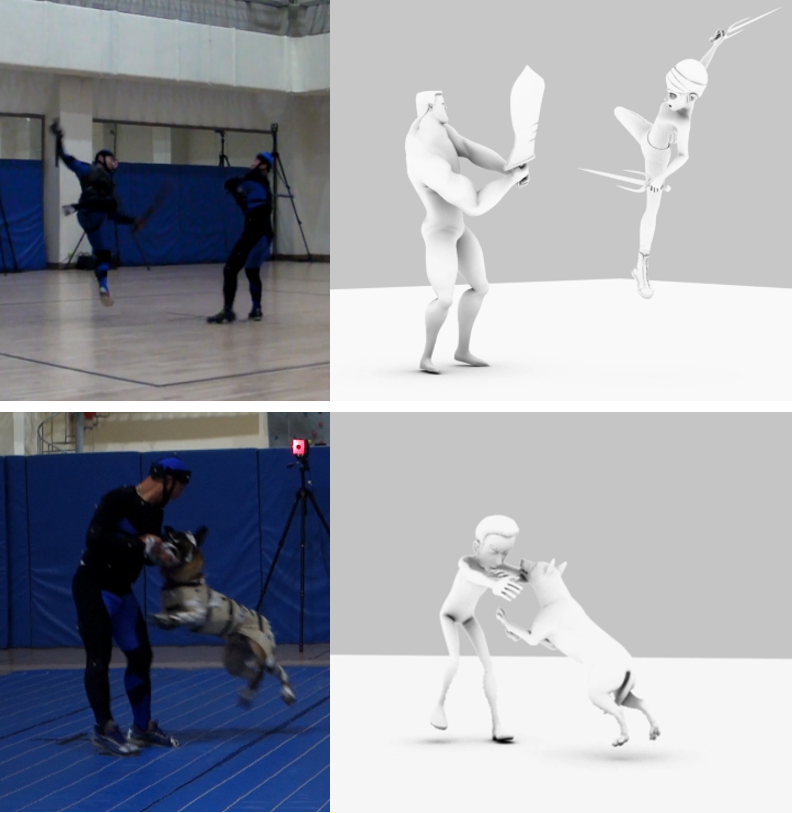
\includegraphics[width=1.0\linewidth]{images/production}
  \caption{Result of our method applied to the animation production pipeline. (Top) Snapshot of two character scene (Bottom) Snapshot of human and dog character scene}
  \label{fig:productionPipeline}
\end{figure}

%\begin{figure*}[ht]
%  \centering
%  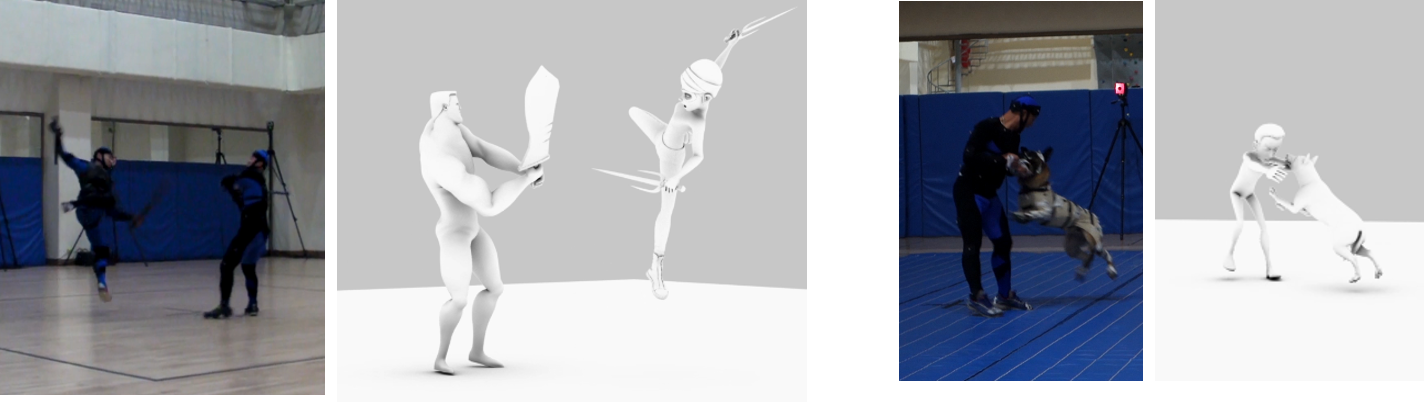
\includegraphics[width=.8\linewidth]{images/productionPipeline}
%  \caption{Result of our method applied to the animation production pipeline. (a) Snapshot of fighting two character scene (b) Snapshot of fighting human and dog character scene}
%  \label{fig:productionPipeline}
%\end{figure*}

%\begin{figure}[!ht]
%    \centering
%    \begin{subfigure}[b]{0.4\textwidth}
%        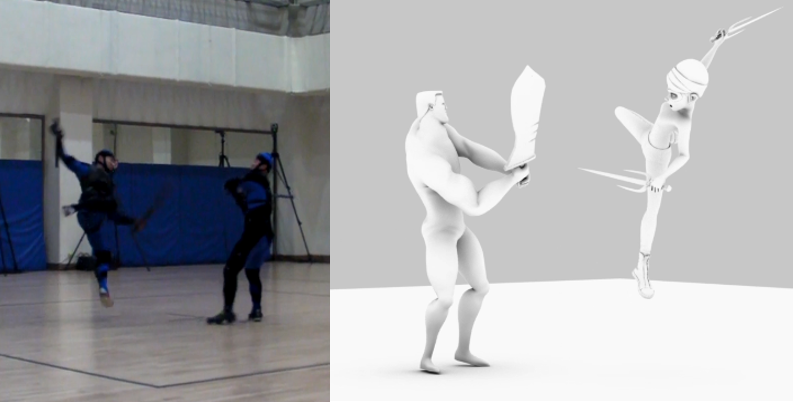
\includegraphics[width=\textwidth]{images/production1}
%        \caption{a}
%    \end{subfigure}
%    %add desired spacing between images, e. g. ~, \quad, \qquad, \hfill etc. 
%      %(or a blank line to force the subfigure onto a new line)
%    \begin{subfigure}[b]{0.4\textwidth}
%        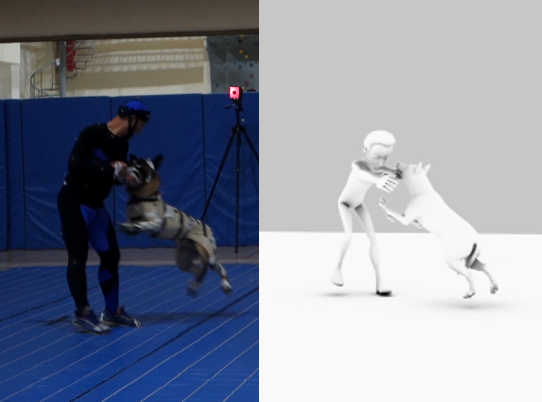
\includegraphics[width=\textwidth]{images/production2}
%        \caption{b}
%    \end{subfigure}
%    
%    \caption{Production Example
%    }
%    \label{fig:productionPipeline}
%\end{figure}

%\begin{table*}[ht]
%  \centering
%  \caption{An average error of different skeleton representation methods.}
%  \begin{tabular}{|b|b b b b b|}
%    \hline
%    Character & Joint Position & Joint Angle & Only Hierarchy & Only Global & Proposed \\
%    \hline
%    character A & & & & &\\
%    character B & & & & & \\
%    character C & & & & & \\
%    character D & & & & & \\
%    \hline
%  \end{tabular}
%\end{table*}
%\newpage
\section{Discussion \& Limitations}

\textbf{Regression-based motion mapping}
There are two different approaches to achieving inverse rig mapping: one is optimization based approach that is similar to our method, and the other is a regression-model-based approach that requires example data.
The benefit of the regression based approach lies in performance because the required runtime computation is simple interpolation of the example data. Thus, this approach can be a good alternative with a sufficient number of high quality examples. 
However, creating the example data is not an easy task. The artist is required to create \textit{good} example motion data per each character rig. The \textit{good} is also hard to define, because the examples should cover the entire range of motion. If the artist provides example data with different rig parameters for a single pose, it may cause conflict in a regression model.
Although real-time performance is an appealing benefit, it is not an essential requirement in the inverse motion mapping because it is one-time process in the production pipeline.
As a future work, it would be a good idea to use a regression model for an unbiased automatic uniform sampling for the entire skeletal configuration that is constrained by the range of motion.

\textbf{Keyframe reduction}
Our optimization results in a dense key frame data because we optimize each pose of character motion.
The dense keyframes are not convenient to edit for an artist, so we perform a keyframe reduction\cite{seol2011artist} for each rig parameter after the motion mapping process. Key pose extraction from motion data is another alternative\cite{halit2011multiscale}.
Both of the methods are applicable in the production pipeline. 

\textbf{Limitations}
If the character rig has full body rig controllers such as full body IK, our rig analysis process cannot group the parameters, because the entire skeletal segments are connected to every rig space parameter.
However, the main purpose of the rig analysis is to increase the efficiency in optimization by dividing the problem into a set of sub-problems.
Therefore, although the full body rig controller can decrease the performance, the mapping can be done without any problem.
Our method successfully maps the motion to rigs even in these cases.

Our optimization is based on the Jacobians of rig and skeletal parameters.
If the skeletal parameter remains unchanged in a specific range of the rig space parameters, our solution can overgrow in the range.
For example, the fully stretched IK end effector controllers(Figure~\ref{fig:limit}, left) and the translational IK pole vector controllers(Figure~\ref{fig:limit}, right) have infinite solutions occurred the specific ranges as indicated by the blue line and the blue plane in Figure~\ref{fig:limit}.
The infinite solution occrued by the use of IK controllers is well known, and it can be simply solved by clamping\cite{buss2004introduction} after the motion mapping. Providing an automatic parameter clamping when parameters have infinite solutions in a specific range can be a direction for future work.

\begin{figure}[!ht]
\centering
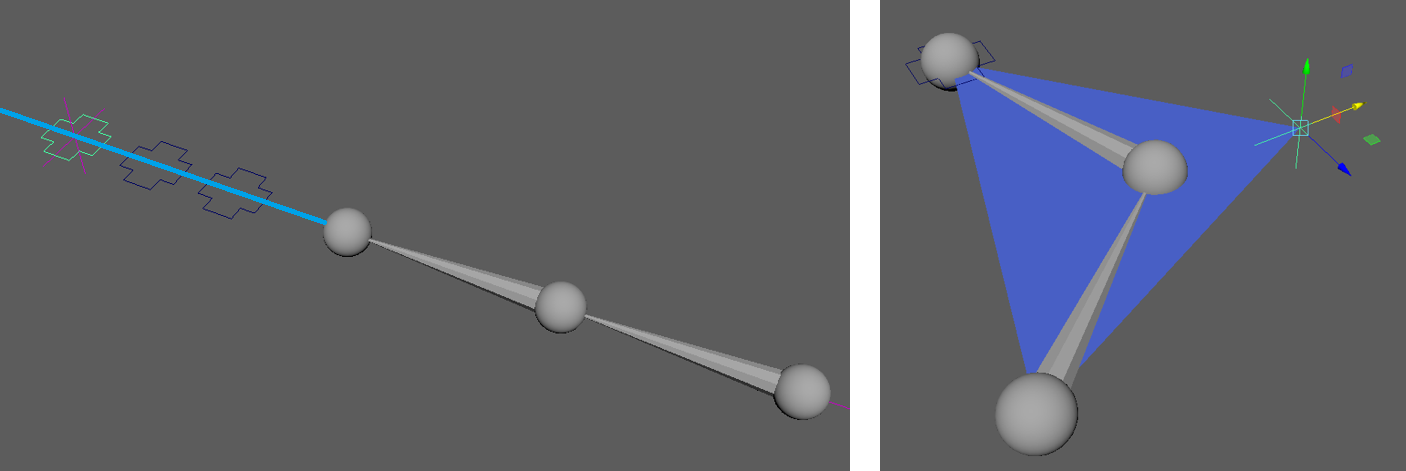
\includegraphics[width=3.0in]{images/ikProblem}
\caption{(left) Fully stretched IK end effector problem (right) IK pole vector controller problem}
\label{fig:limit}
\end{figure}

%\newpage

\section{Conclusions}
We propose an inverse mapping method from motion data to a general character rig based on a spacetime optimization.
%Our method can be seamlessly applied to the current production pipeline.
As the rig space is a highly abstract user interface, the goal of our algorithm is to provide a robust mapping method without any prior information.
%The contributions of our method are two-fold: 
%The v a robust mapping method which does not require any manual sepcification or prior data.
In addition, we propose a new skeletal representation based on the Lie group 3D transformations of the rigid body, which helps achieve improved error minimization during the  optimization process.
%We prpose a new skeletal representation based on the Lie group 3D transformations of rigid body, which provides accurate error minimization during our optimization process.
We showed the stability and the generality of our method through various results.
Since our method can be seamlessly applied to the current production pipeline, it can increase the productivity of animation production remarkably.





\bibliographystyle{acmsiggraph}
\nocite{*}
\bibliography{template}

\appendix
\section{Detailed shape of matrices and vectors in the optimization} \label{App:AppendixA}
% the \\ insures the section title is centered below the phrase: AppendixA
We provide a detailed shape of vectors and matrices in the optimization process(section \ref{objectiveFunction}).
The matrices are represented as:
\begin{gather*}
\boldsymbol{J} =
\begin{bmatrix}
\mathbf{J}(t_1) & \dots & 0\\ 
\vdots & \ddots &  \vdots \\ 
0 & \dots & \mathbf{J}(t_n)
\end{bmatrix},
\boldsymbol{A} = \begin{bmatrix}
0 &  & \cdots &  & 0 \\ 
\mathbf{I} & -2\mathbf{I} & \mathbf{I} &  & \\ 
\vdots &  &\ddots  &  & \vdots\\ 
 &  &  \mathbf{I}& -2\mathbf{I} & \mathbf{I}\\ 
0 &  &  &  & 0 
\end{bmatrix},\\ 
\boldsymbol{K}_{h} = \begin{bmatrix}
\mathbf{K}_{h}(t_1) &  \cdots & 0 \\ 
\vdots & \ddots & \vdots \\ 
0 & \cdots & \mathbf{K}_{h}(t_n)
\end{bmatrix},\\
\boldsymbol{K}_{s} = \begin{bmatrix}
\mathbf{K}_{s}(t_1) & \cdots  & 0 \\ 
\vdots & \ddots & \vdots \\ 
0 & \cdots & \mathbf{K}_{s}(t_n)
\end{bmatrix},\\
\boldsymbol{L} = \begin{bmatrix}
\mathbf{L}(t_1) & \cdots  & 0 \\ 
\vdots & \ddots & \vdots \\ 
0 & \cdots & \mathbf{L}(t_n)
		\end{bmatrix},\\
\mathbf{L}(t_i) = \lambda(t_i)\begin{bmatrix}
\left | \Delta c_{1}(t_i)  \right |   & \cdots &0 \\ 
\vdots & \ddots & \vdots \\ 
0 & \cdots & \left | \Delta c_{n}(t_i)  \right |
\end{bmatrix}^{-1},
\end{gather*}

The vectors are represented as:
\begin{equation}
\begin{split}
\Delta\boldsymbol{C} &= \left ( \Delta\mathbf{c}(t_1),\Delta\mathbf{c}(t_2),...,\Delta\mathbf{c}(t_n) \right )^{T},\\
\Delta\boldsymbol{S} &= \left ( \Delta\mathbf{s}(t_1),\Delta\mathbf{s}(t_2),...,\Delta\mathbf{s}(t_n) \right )^{T},\\
\boldsymbol{H} &= \left ( \mathbf{h}(t_1),\mathbf{h}(t_2),...,\mathbf{h}(t_n) \right )^{T},\\
\boldsymbol{Z} &= \left ( z(t_1),z(t_2),...,z(t_n) \right )^{T}.
\end{split} \notag
\end{equation}




\end{document}
